\documentclass[specialist,
               substylefile = spbu_report.rtx,
               subf,href,colorlinks=true, 12pt]{disser}

\usepackage[a4paper,
            mag=1000, includefoot,
            left=3cm, right=1.5cm, top=2cm, bottom=2cm, headsep=1cm, footskip=1cm]{geometry}
\usepackage[T2A]{fontenc}
\usepackage[utf8]{inputenc}
\usepackage[english,russian]{babel}
\ifpdf\usepackage{epstopdf}\fi

% Точка с запятой в качестве разделителя между номерами цитирований
%\setcitestyle{semicolon}


% Включать подсекции в оглавление
\setcounter{tocdepth}{2}

\graphicspath{{fig/}}

%----------------------------------------------------------------
\begin{document}

%
% Титульный лист на русском языке
%

% Название организации
\institution{%
    Санкт-Петербургский государственный университет \\
    Прикладная математика и информатика \\
    (для первого курса - Прикладная математика, информатика и искусственный интеллект)
}

\title{ Отчет по учебной практике 1 (научно-исследовательской работе) (семестр 1)}

% Тема
\topic{\normalfont\scshape%
Cравние на синтетических данных и на данных с Kaggle методов для рассчёта доверительных интервалов для 90, 99 квантилей}

% Автор
\author{Кривоносов Тимофей Игоревич, группа 22Б05-мм}

% Научный руководитель

\sastatus {Р.\,Н.~Мокаев \newline д.\,ф.-м.\,н. \newline Краткий отзыв:}
\sa  {Кафедра ПРИКЛАДНОЙ КИБЕРНЕТИКИ Санкт-Петербургий государственный университет Математико-механический факультет}



% Город и год
\city{Санкт-Петербург}
\date{\number\year}

\maketitle

\newpage
\section{ОТЗЫВ}

\newpage
\tableofcontents
\newpage

\section{ВВЕДЕНИЕ}
В современном мире статистический анализ играет важную роль во многих областях, от науки до бизнеса. При работе с данными мы часто сталкиваемся с необходимостью оценки параметров и построения доверительных интервалов для различных квантилей распределений. Квантили представляют собой значения, разделяющие вероятностное распределение на равные части.

В данной курсовой работе мы сосредоточимся на сравнении методов для расчета доверительных интервалов для 90-го и 99-го квантилей на основе синтетических данных и данных, предоставленных платформой Kaggle. Синтетические данные являются созданными искусственным образом наборами данных, которые позволяют нам контролировать различные аспекты, такие как распределение, объем выборки и т.д. Данные, полученные с Kaggle, представляют собой реальные данные, предоставленные сообществом пользователей этой платформы.
\subsection{Задачи}
Для синтезирования данных и проверки методов поиска доверительных интервалов для 90 и 99 квантилей в задаче сравнения производительности и задержки (latency). Решено 2 задачи:  Page loading" на синтаксических данных и маркетинговая задача на данных из  Kaggle.
\begin{itemize}

\item Подготовить данные: Создать выборки из результатов тестов для маркетинговой задачи. Использовать dataset, предоставленный интернет сообществом. Также создать тестовые данные для задачи "Page loading problem", так как зачастую невозможно получить реальные данные, поскольку это является коммерческой тайной.а
\item Анализировать выборки: Используйте статистические методы для анализа выборок и вычисления доверительных интервалов. Для нахождения доверительного интервала 90\% квантили, найдите 5-й и 95-й перцентили выборки. Для доверительного интервала 99\% квантили найдите 0.5-й и 99.5-й перцентили выборки.

\item  Проверьте методы поиска доверительных интервалов: Сравните результаты, полученные различными методами поиска доверительных интервалов. Убедитесь, что методы возвращают адекватные и интерпретируемые результаты.

\item Интерпретация результатов: Проанализируйте полученные доверительные интервалы и сделайте выводы относительно производительности и задержки системы. Например, если интервалы значительно отличаются для двух методов, это может указывать на значимые различия между ними.
\end{itemize}

Основной целью нашего исследования является провести сравнительный анализ методов расчета доверительных интервалов для выбранных квантилей на основе обоих типов данных. Это позволит нам оценить, насколько точно и надежно эти методы работают в различных условиях и с разными типами данных.

Ожидается, что результаты данного исследования помогут нам лучше понять применимость и эффективность различных методов для расчета доверительных интервалов на основе разных типов данных, что может быть полезным при принятии статистических решений в реальных ситуациях.

\newpage
\section{ОСНОВНАЯ ЧАСТЬ}
Доверительные интервалы являются важным инструментом в статистике и анализе данных. Они предоставляют информацию о диапазоне значений, в пределах которого с определенной вероятностью находится истинное значение параметра популяции. Методы нахождения доверительных интервалов разрабатываются для различных статистических оценок, таких как среднее, медиана, квантили и дисперсия.

В данном контексте существует несколько методов, включая аналитические, bootstrap и другие. Аналитические методы обычно требуют явных аналитических моделей и предположений о распределении данных. Bootstrap- это метод ресемплинга, который позволяет оценивать доверительные интервалы на основе эмпирических данных без явных предположений.

В этом контексте, мы будем исследовать различные методы нахождения доверительных интервалов и сравнивать их производительность в оценке статистических параметров в задачах анализа производительности и задержки.

\subsection{Наивный подход}

Наивный подход (или иногда "классический подход") при поиске доверительного интервала предполагает использование простых формул или методов для оценки параметров популяции или статистических характеристик на основе имеющихся данных без учета сложных статистических моделей или методов ресемплинга.

Основные черты наивного подхода:
\begin{itemize}
    \item Простота: Наивный подход обычно предполагает использование простых статистических оценок, таких как выборочное среднее, выборочная дисперсия, медиана и квантили, без необходимости в более сложных методах.
    \item Явные формулы: В большинстве случаев наивные методы имеют явные аналитические формулы для вычисления оценок и доверительных интервалов. Например, доверительный интервал для среднего значения в выборке с известной дисперсией может быть вычислен с использованием формулы Z-критерия.
    \item Предположения о распределении: Наивные методы часто основываются на предположениях о распределении данных, таких как нормальное распределение. Они могут быть неустойчивыми к нарушениям этих предположений.
    \item Ограниченная гибкость: Наивные методы могут быть ограничены в способности учитывать сложные зависимости в данных или рассматривать данные, не подчиняющиеся стандартным распределениям.
\end{itemize}

Наивный подход полезен, когда у вас есть хорошие основания для использования простых методов, и когда они дают приемлемые результаты. Однако в случае сложных данных или данных, не соответствующих предполагаемым распределениям, наивный подход может быть недостаточным и неустойчивым. В таких случаях более сложные методы, такие как bootstrapили аналитические модели, могут быть более надежными.

Алгоритм нахождения доверительного интервала с его помощью обычно включает следующие шаги:
\begin{itemize}
    \item Шаг 1: Собрать выборку данных. Это могут быть измерения, результаты эксперимента или другие данные, на основе которых вы хотите построить доверительный интервал.
    \item Шаг 2: Выбрать уровень доверия (например, 95 \% или 99\%). Уровень доверия определяет, с какой вероятностью истинное значение параметра популяции находится внутри доверительного интервала.
    \item Шаг 3: Определить статистическую оценку параметра. Наивный подход часто использует выборочные статистики, такие как выборочное среднее $\bar{x}$ или выборочная медиана, для оценки параметра популяции.
    \item Шаг 4: Определить стандартную ошибку. Стандартная ошибка (SE) измеряет разброс выборочной статистики и зависит от объема выборки. Для среднего значения это может быть вычислено как стандартное отклонение выборки, деленное на корень из размера выборки ($SE = \sigma / \sqrt{n} $, где $\sigma$ - стандартное отклонение популяции).
    \item Шаг 5: Определить критическое значение. Критическое значение определяет, какие значения статистики считаются "достаточно экстремальными" для данного уровня доверия. Наивный подход обычно использует критические значения из стандартных распределений, таких как Z-распределение или t-распределение.
    \item Шаг 6: Вычислить доверительный интервал. Доверительный интервал определяется как оценка параметра плюс/минус критическое значение, умноженное на стандартную ошибку. Для среднего значения (наивный метод):
    
    Доверительный интервал = оценка параметра ± (критическое значение * SE)

\end{itemize}

Пример:

Предположим, у нас есть выборка из 30 измерений длины стержня, и мы хотим построить 95 \% доверительный интервал для средней длины стержня. Стандартное отклонение выборки равно 2 см.

\begin{itemize}
    \item Выборка данных: [10, 11, 12, 14, 15, 11, 13, 12, 14, 15, 15, 13, 12, 13, 14, 16, 17, 18, 15, 12, 13, 12, 14, 15, 16, 17, 16, 13, 12, 14]
    \item Уровень доверия: 95\%
    \item Статистическая оценка: Выборочное среднее $bar{x}$ = 14
    \item Стандартная ошибка: $SE = 2 / \sqrt{30} \approx 0.365$
    \item Критическое значение: Для 95\% доверия с использованием Z-распределения, критическое значение равно примерно 1.96.
    \item Вычисление доверительного интервала: 
    
    Доверительный интервал = 14 ± (1.96 * 0.365)$ \approx $ [13.29, 14.71]
    \end{itemize}
    Таким образом, с 95\% уровнем доверия мы можем утверждать, что средняя длина стержня находится в интервале от 13.29 см до 14.71 см.

\subsection{Bootstrap}
Bootstrap- это метод статистической ресемплинга, который используется для оценки дисперсии и доверительных интервалов для статистических оценок, когда точное аналитическое решение сложно или невозможно. Он широко применяется в статистике и машинном обучении для решения различных задач, таких как оценка параметров, построение доверительных интервалов и проверка гипотез. Вот как он работает:
\begin{itemize}
    \item Создание репликаций: Из вашей исходной выборки размером N (обычно с заменой) генерируются множество новых выборок (репликаций). Количество репликаций, обычно обозначаемое как B, может быть выбрано пользователем и обычно составляет несколько сотен или тысяч.
    \item Оценка интересующей статистики: Для каждой из B репликаций, вы оцениваете интересующую вас статистику. Это может быть, например, среднее, медиана, доля, стандартное отклонение, коэффициент корреляции или что-либо еще в зависимости от вашей задачи.
    \item Анализ распределения: После оценки статистики для каждой репликации, вы получаете распределение значений этой статистики на основе бутстрэп -выборок.
    \item Построение доверительных интервалов: Из анализа этого распределения можно построить доверительные интервалы для вашей статистики. Наиболее распространенным методом для этого является метод "перцентильного доверительного интервала", который использует квантили распределения.
\end{itemize}
Пример использования метода:
\newline
Предположим, у нас есть выборка размером 100 наблюдений и мы хотим построить доверительный интервал для среднего значения. Мы можем применить метод bootstrapследующим образом:

\begin{itemize}
    \item Создаем множество бутстрэп-выборок путем случайного выбора 100 наблюдений из исходной выборки с возвращением.
    \item Для каждой бутстрэп-выборки вычисляем среднее значение.
    \item Полученные средние значения образуют распределение, которое отражает неопределенность вокруг истинного среднего значения.
    \item Используем полученное распределение для построения доверительного интервала, например, 95\% доверительного интервала будет содержать средние значения, лежащие между 2.5-м и 97.5-м процентилями этого распределения.
\end{itemize}

Таким образом, метод bootstrapпозволяет оценить статистическую неопределенность и построить доверительные интервалы для различных параметров на основе анализа повторных выборок из исходной выборки.

\subsection{Дельта подход}

Дельта-метод - это статистический метод, используемый для оценки дисперсии и построения доверительных интервалов для функций случайных величин на основе их оценок и производных. Основное предположение метода Дельта состоит в том, что оценки параметров близки к нормальному распределению.


Доказательство метода Дельта является более сложным и требует математической формализации и использования разложения в ряд Тейлора. Давайте представим общий контур доказательства метода Дельта, который включает следующие шаги:

Предположим, у нас есть функция случайной величины X, которую мы обозначим как g(X), и мы хотим оценить ожидание этой функции, то есть E[g(X)].

\begin{itemize}
    \item Разложение в ряд Тейлора: Начнем с разложения в ряд Тейлора для функции g(X) вокруг некоторого фиксированного значения a. Это разложение будет иметь вид:
    
    $g(X) = g(a) + g'(a)(X - a) + g''(a)(X - a)^2/2 + ...$
    где g'(a) представляет производную функции g(X) в точке a.
    \item Взятие ожидания: Теперь возьмем ожидание от обеих сторон уравнения:
    
    $E[g(X)] = E[g(a) + g'(a)(X - a) + g''(a)(X - a)^2/2 + ...]$
    \item Использование линейности ожидания: Ожидание линейно, поэтому мы можем разбить его на отдельные члены:
    
    $E[g(X)] = g(a) + E[g'(a)(X - a)] + E[g''(a)(X - a)^2/2] + ...$
    \item Оценка среднего и дисперсии: Мы видим, что первый член g(a) - это константа, и остальные члены представляют собой смешанные моменты случайной величины X. Мы можем использовать оценки математического ожидания и дисперсии для оценки E[g(X)]:
   
    $E[g(X)] \approx g(a) + g'(a)E(X - a) + (1/2)g''(a)E((X - a)^2)$
    \item Замена параметров: Теперь мы заменяем параметры a, g(a), g'(a) и g''(a) на их оценки, соответственно. Обозначим оценки как $\widehat{a}$, $g(\widehat{a})$, $g'(\widehat{a})$ и $g''(\widehat{a})$:
    
    $E[g(X)] \approx g(\widehat{a} ) + g'(\widehat{a})E(X - \widehat{a}) + (1/2)g''(\widehat{a})E((X - \widehat{a})^2)$
    \item Оценка дисперсии: Мы можем оценить дисперсию случайной величины $X - \widehat{a}$ и заменить $E((X - \widehat{a})^2)$ на $Var(X - \widehat{a})$:
    
    $E[g(X)] \approx g(\widehat{a}) + g'(\widehat{a})E(X - \widehat{a}) + (1/2)g''(\widehat{a})Var(X - \widehat{a})$
    \item Итоговый результат: Таким образом, мы получаем оценку E[g(X)] в зависимости от оценок параметров функции g(X), а также смешанных моментов и дисперсии случайной величины $X - \widehat{a}$.
    Это представляет собой общий контур доказательства метода Дельта, который объясняет, как мы можем оценить математическое ожидание функции случайной величины, используя разложение в ряд Тейлора и оценку параметров функции и их производных.
\end{itemize}

Чтобы использовать метод Дельта для квантильных метрик (например, для оценки доверительного интервала квантиля), выполните следующие шаги:

\begin{itemize}
\item Оцените квантиль на основе вашей выборки. Обозначьте это значение как оценку квантиля (например,$ \widehat{q}$).
\item Вычислите производную функции квантиля по параметру распределения (обычно параметр p). Это даст вам информацию о градиенте функции вблизи оценки квантиля.
\item Вычислите значение производной в точке, соответствующей вашей оценке квантиля (например, $\widehat{q}(p)$). Это будет вашей оценкой производной.
\item Вычислите дисперсию оценки квантиля, $Var(\widehat{q})$.
\item Теперь, используя метод Дельта, можно вычислить доверительный интервал для оценки квантиля:
\item 
    Нижняя граница интервала: $\widehat{q} - Z * sqrt(Var(\widehat{q}))$

    Верхняя граница интервала: $\widehat{q} + Z * sqrt(Var(\widehat{q}))$
\end{itemize}
Здесь Z - это критическое значение для выбранного уровня доверия (например, для 95\% уровня доверия, $Z  \approx 1.96$).

 \textit{Более углубленно дельта метод и пример его использования представлен в приложении 2 [\ref{sec: Приложение 2}]}

Метод Дельта позволяет оценивать дисперсию и строить доверительные интервалы для различных функций от случайных величин, включая квантили. Это полезный метод в статистике и анализе данных, который позволяет оценить не только средние значения, но и другие статистики и метрики с учетом их дисперсии и нормальности распределения.



\newpage
\section{Page loading Problem}
    \subsection{Описание задачи и переменных}
    Сравнивать методы будем в популярной задаче поиска средней скорости загрузки веб страницы. 
    Существует один важный тип метрик, который не может быть хорошо обобщен в среднем, это показатели производительности (например, время загрузки страницы). 
    Представьте себе два веб-сайта с точно таким же средним временем загрузки страницы 0,5 секунды. 
    Веб-сайт A загружает все страницы за 0,5 с, в то время как веб-сайт B загружает 10  \% страниц за 5 с, а оставшиеся 90 \% страниц за 0.
    Несмотря на то же самое среднее время загрузки страницы 0,5 с, веб-сайт A будет восприниматься как быстро, 
    потому что каждая страница загружается в мгновение ока, в то время как веб-сайт B будет восприниматься как медленный,
    потому что пользователям часто приходится ждать 5 секунд, прежде чем страница загружается.
    Поэтому, чтобы оптимизировать скорость работы сайта для участников LinkedIn, 
    нам нужно сократить время загрузки самой медленной загрузки страницы, вместо того, чтобы сокращать среднее время 
    загрузки страницы, делая быстрые страницы еще быстрее. Отраслевой стандарт для измерения времени загрузки страницы - это квантили,
    такие как 90-й процентиль и 99-й процентиль.

    Предположим, что A/B-тест задается с несколькими вариантами (Kohavi et al., 2013b), где кандидаты в каждом варианте получают разный опыт.
    Мы заинтересованы в измерении того, как опыт в каждом варианте влияет на q-й квантиль времени загрузки страницы. 
    Чтобы измерить это влияние и вычислить статистическую значимость, нам нужны оценки количества выборки и стандартного отклонения квантиля выборки в каждом варианте.
    
    Положим:

        Участники $i = 1,2,3,  ... , n$

        Страници просмотренные i-ым участником $j = 1, 2, 3, ... ,\textit{P}{i}$, где $\textit{P}{i}$ (i.i.d) случайные значения удовлетворяющие функции распрелеления $\mathcal{P}$.

        Загрузка j-ой страницы i-ым участником = $\textit{X}{ij}$   

        q-ый выборочный квантиль $\{\textit{X}{ij}, i = 1,2,...n; j = 1,2,3, ... ,  \textit{P}{i} \}$ обозначим как $\widehat{Q}$ 

        Дисперсия - $Var(\widehat{Q} )$; стандартное откланение $stddev(\widehat{Q})$

    
    \subsection*{Использование методов на тестовых данных}
        
        Создадим Xij, важно заметить, что в решение задачи нас не интересуют пусты строки (это просто значит, что никто не заходид на j-ую страницу)
        

        \begin{figure}[h]
            \centering
            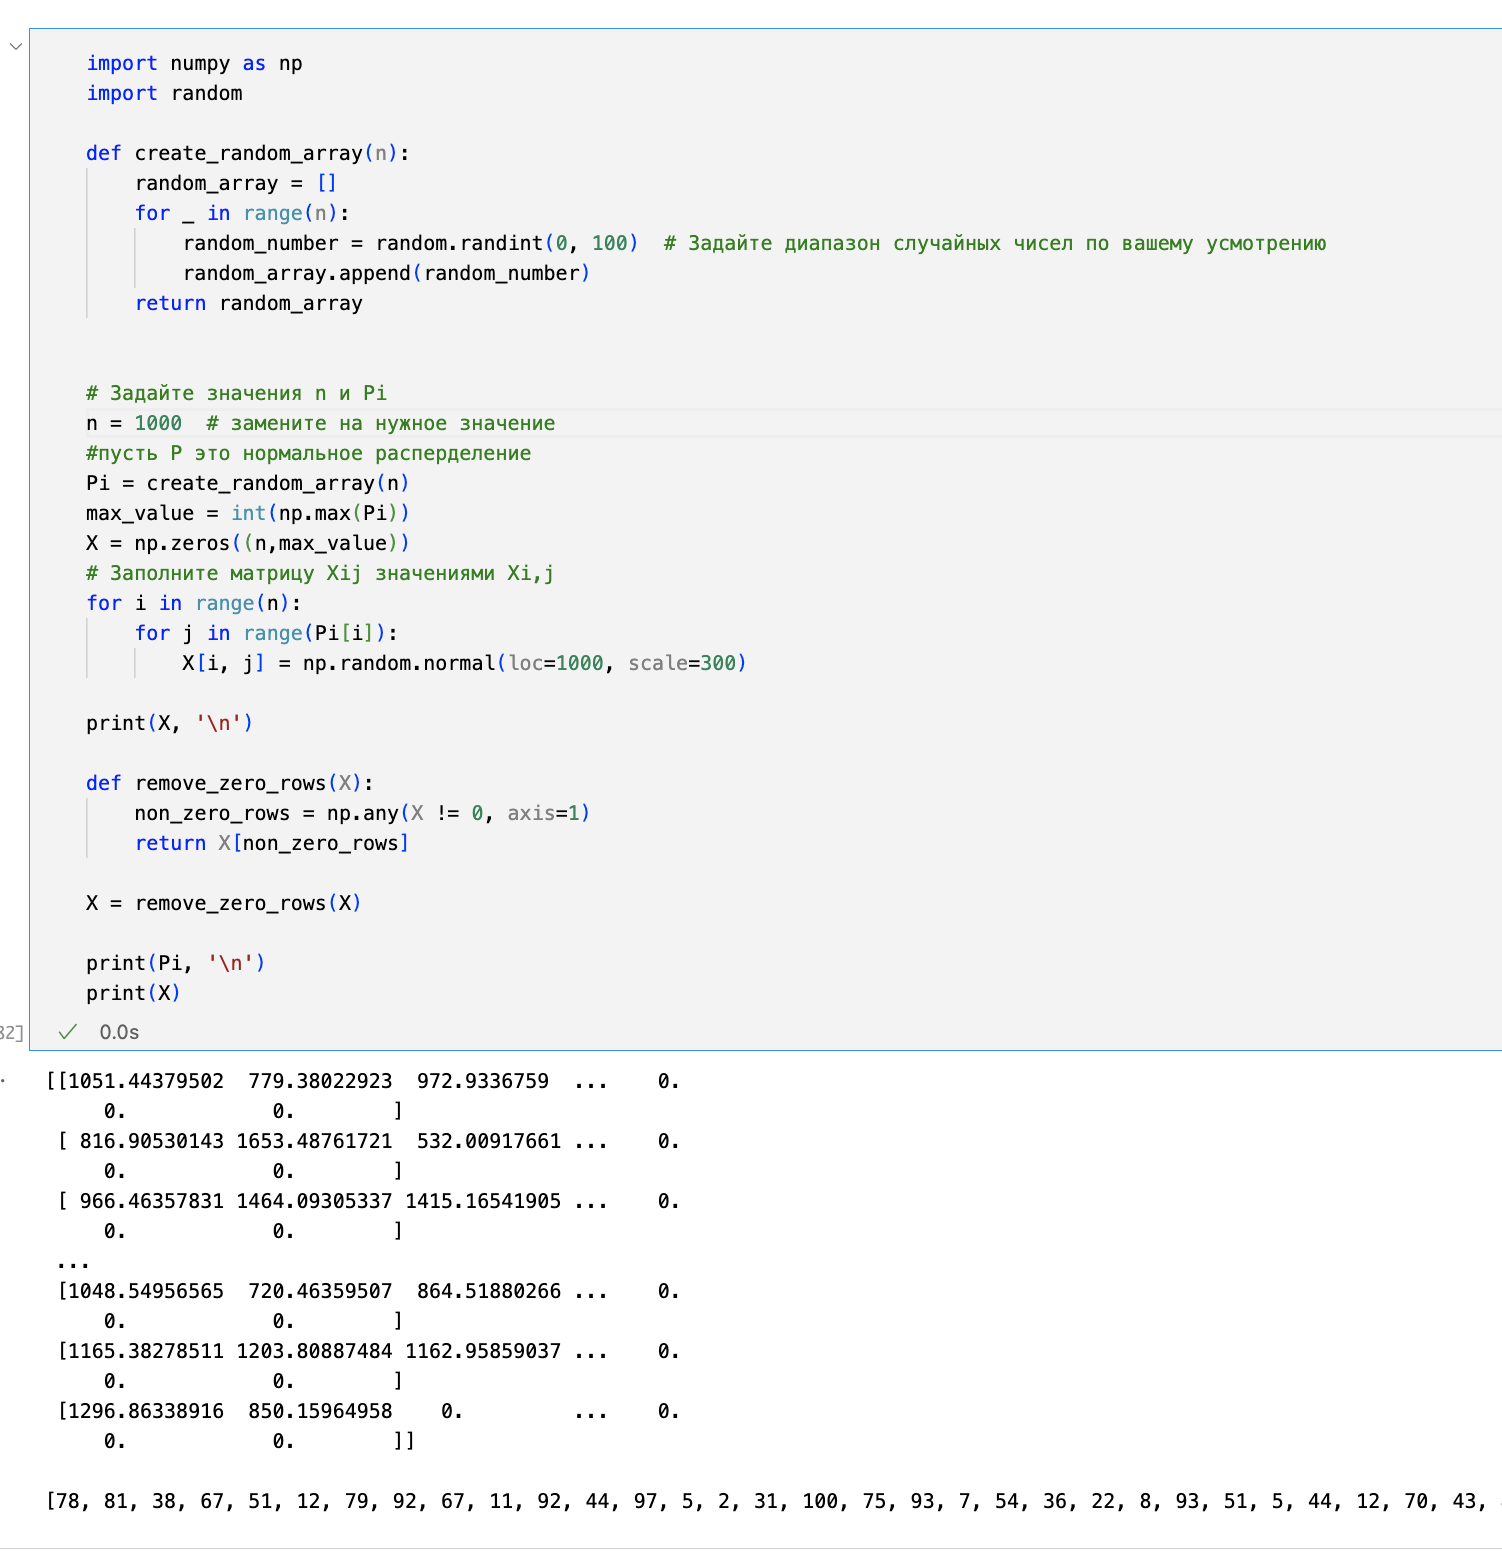
\includegraphics[width=6in]{/Users/krivonosovti/Курсач/Course_Work/Снимок экрана 2023-10-29 в 00.31.05.png}
            \caption{Cоздание тестовых данных}
        \end{figure}
        
       

        \textbf{Наивный подход} 
        Попробуем решить задачу наивынм подходом, для этого просто посичтаем доверительный интервал для каждой страницы, нам известно, что распределение нормальное. Следовательно трудностей не возникнет. 


        \begin{figure}[h]
            \centering
            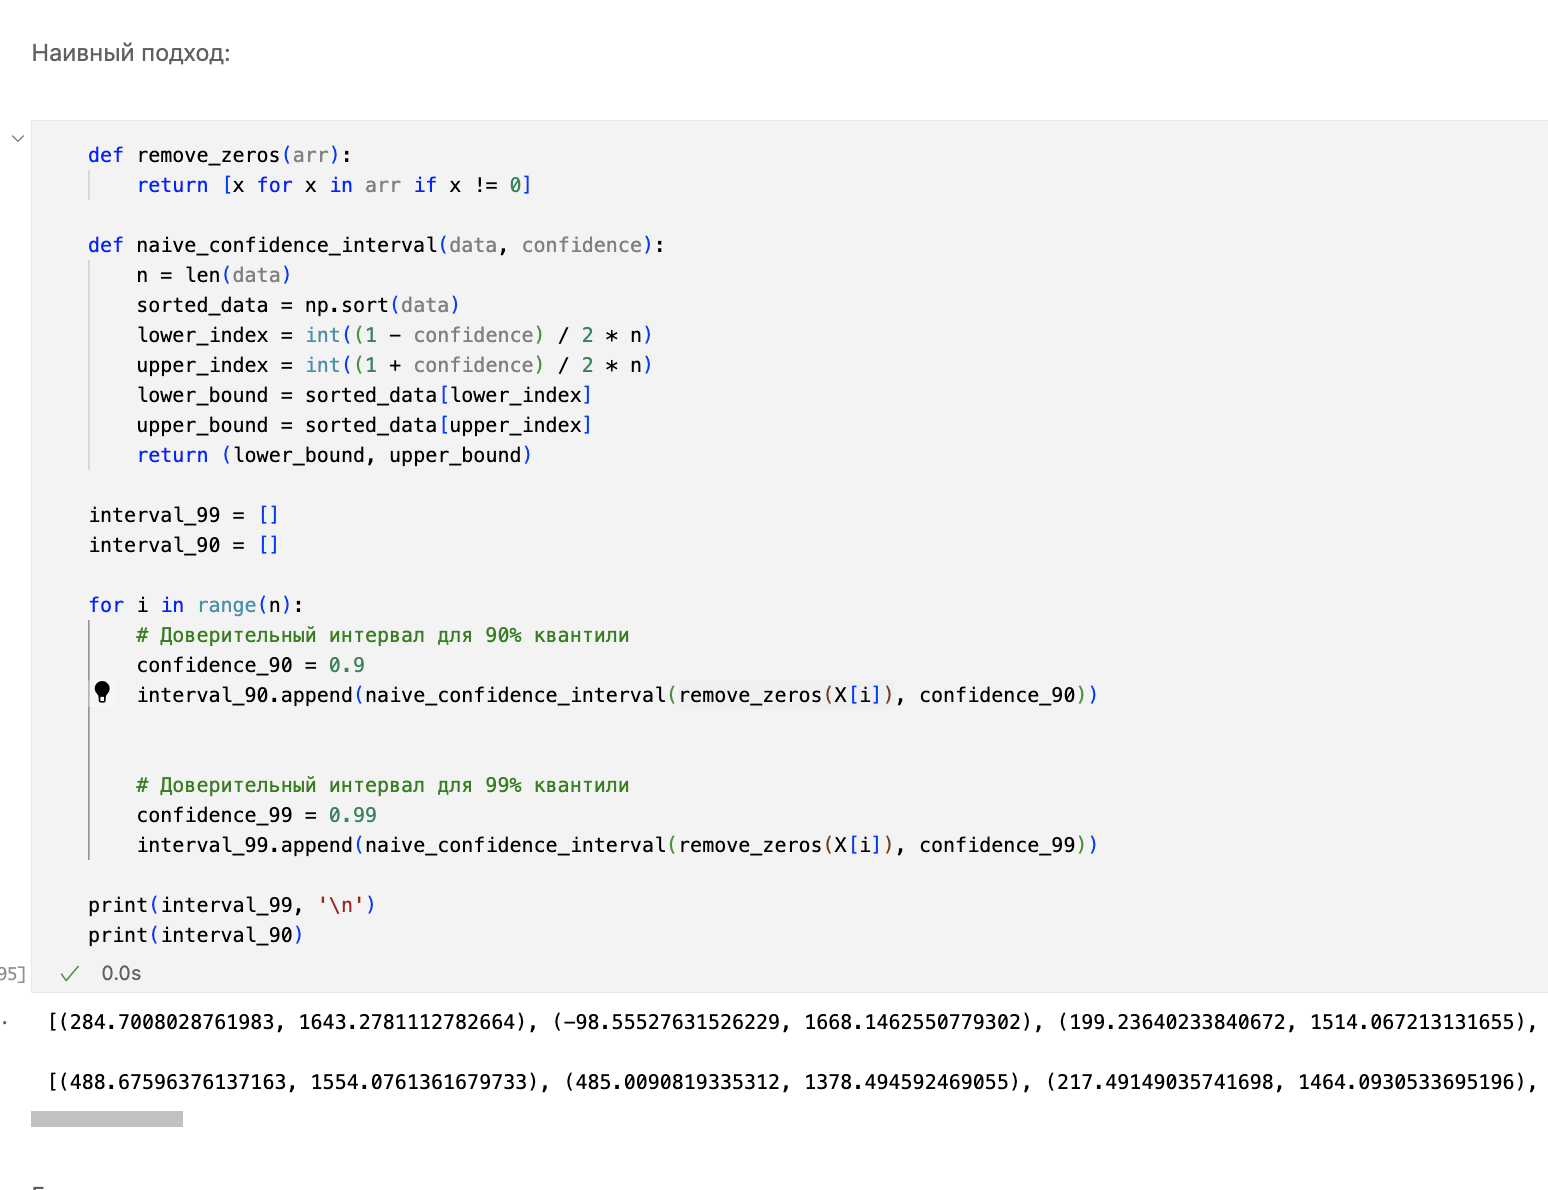
\includegraphics[width=6in]{/Users/krivonosovti/Курсач/Course_Work/Снимок экрана 2023-10-29 в 00.31.35.png}
            \caption{Наивный подход}
        \end{figure}
        
        
        \textbf{Бутстрэп}
        Поскольку времена загрузки страниц для одного и того же пользователя не обязательно являются независимыми, но пользователи в целом независимы, перечисление в методе bootstrap должно происходить на уровне отдельных пользователей, 
        чтобы сохранить структуру зависимости. В k-ой подвыборке бутстрэпа случайным образом выбираются с повторениями n 
        пользователей из исходных n пользователей, затем вычисляется q-ый квантиль времени загрузки страницы для n 
        выбранных пользователей и получается $ \widehat{Q}^{(k)}$. Этот процесс повторяется B раз, и выборочное среднее и выборочная
        дисперсия ${\widehat{Q}^{(k)}; k = 1, 2, . . . , B}$ являются несмещенными оценками $\widehat{Q}$  и $var(\widehat{Q})$(Efron, 1979). Выборочное 
        стандартное отклонение является смещенной оценкой $stddev(\widehat{Q})$, но относительное смещение имеет порядок $O(1)$(Bolch, 1968), поэтому для типичного A/B-теста,
        в котором есть как минимум тысячи выборок, смещение практически равно 0. Рисунок 1 и 2 показывает пример распределения 
        не независимых времен загрузки страницы и распределение bootstrap90-го перцентиля, по которому можно оценить stddev$(\widehat{Q})$.
        Красная пунктирная линия на рисунке 2 представляет собой функцию плотности вероятности подогнанного нормального распределения.

    
        \begin{figure}[h]
            \centering
            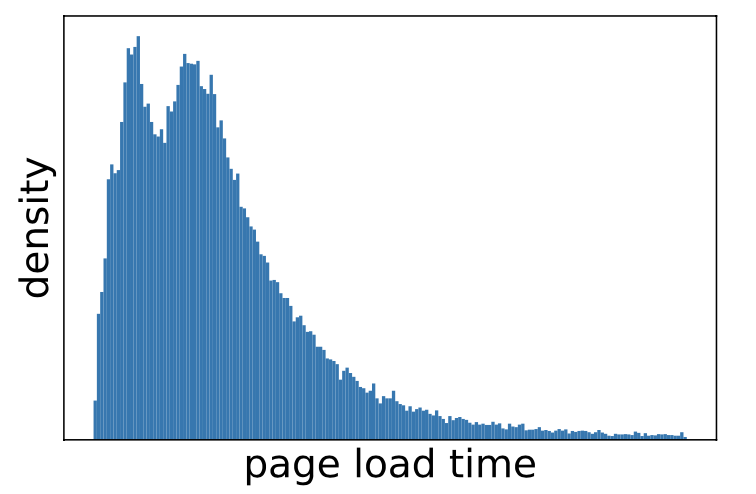
\includegraphics[width=0.5\textwidth]{Снимок экрана 2023-10-26 в 19.21.39.png}
            \caption{(A) Распределение времени загрузки страниц, не относящихся к i.i.d.}
        \end{figure}
        
        \begin{figure}[h]
            \centering
            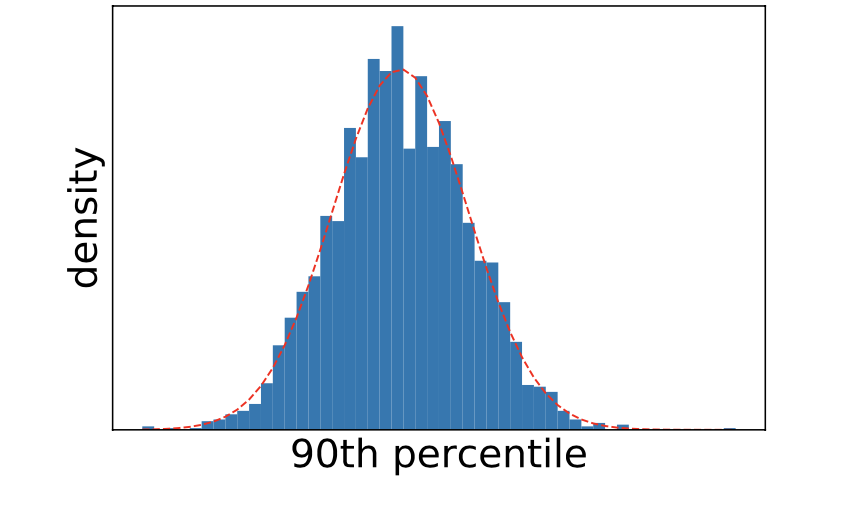
\includegraphics[width=0.5\textwidth]{Снимок экрана 2023-10-26 в 19.21.35.png}
            \caption{(B) Распределение 90-х процентилей начальной загрузки}
        \end{figure}


            
        \begin{figure}[h]
            \centering
            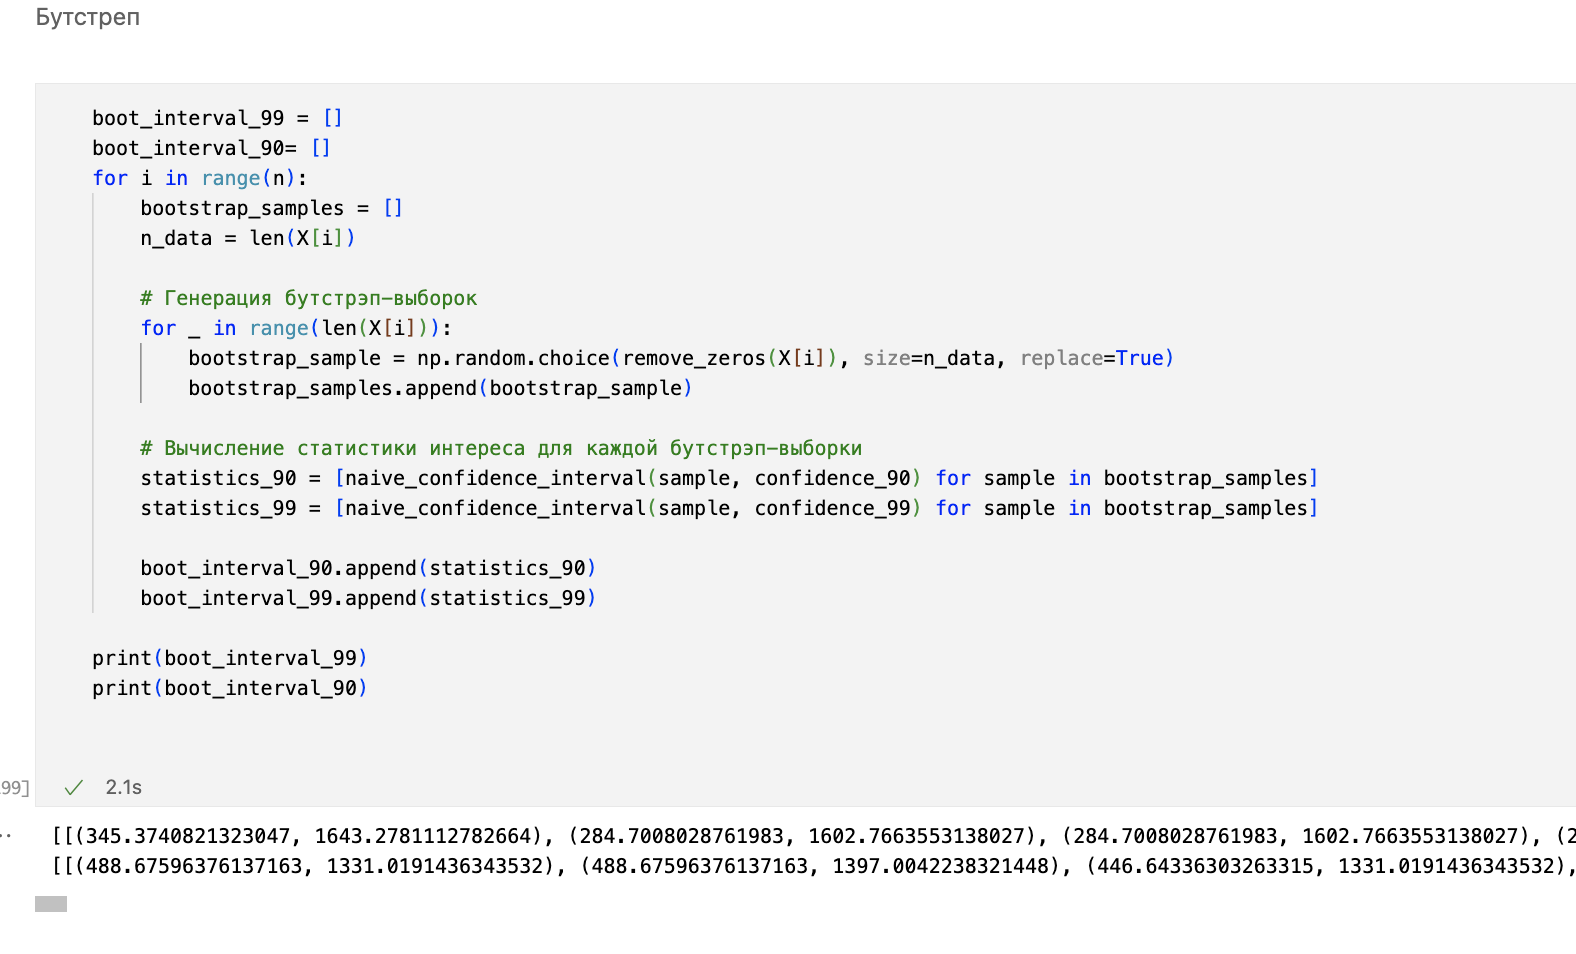
\includegraphics[width=5in]{/Users/krivonosovti/Курсач/Course_Work/Снимок экрана 2023-10-29 в 00.31.45.png}
            \caption{Будстрэп для задачи поиска CI 90 и 99 квантиля скорости загрузки страницы}
        \end{figure}
        

        \textbf{Дельта метод}
        \textit{Более развернуто дельта метод представлен в приложении 1 [\ref{sec: Приложение 1}]} 
        
        Тут мы не будем сильно углубляться в математическую составляющую. 
        
        Прежде чем перейти к деталям предложенной методологии, важно отметить, что нам требуется: статистическая 
        достоверность и масштабируемость. Чтобы принимать правильные решения на основе результатов A/B-тестирования, 
        оценки квантилей выборки и стандартного отклонения должны быть достоверными; одновременно быстрый цикл инноваций 
        продукта требует, чтобы алгоритм был масштабируемым для обработки результатов A/B-тестов на 300 миллиардах строк 
        входных данных ежедневно и завершал вычисления за несколько часов или быстрее.

        Чтобы установить действительную и масштабируемую оценку стандартного отклонения квантиля независимых выборок, мы надеемся, 
        что асимптотическое распределение замкнутой формы может быть установлено с помощью центральной предельной теоремы 
        (van der Vaart, 2012). Выражение закрытой формы освободит нас от начальной загрузки и позволит избежать трудоемкого 
        процесса повторной выборки. Тот факт, что квантовое распределение начальной загрузки на Рис. 4 хорошо 
        соответствует нормальному распределению, настоятельно говорит о том, что такое асимптотическое распределение 
        действительно существует.

        Одно из ключевых наблюдений, которое повысило эффективность алгоритма, заключается в том, 
        что нам необходимо учитывать только тех пользователей, у которых действительно был просмотр страницы для расчета 
        стандартного отклонения. В контексте триггерного анализа (Kohavi and Longbotham 2017), популяция эксперимента 
        включает всех участников, удовлетворяющих триггерному условию (например, посещение LinkedIn). Однако не все 
        участники этой группы просматривали конкретную страницу (например, Страницу вакансий), для которой мы хотим 
        измерить влияние времени загрузки страницы. Мы показываем, что для оценки дисперсии квантиля необходимо учитывать 
        только тех участников, которые просматривали интересующую страницу. Это значительно сокращает объем хранения и 
        вычислений, особенно при низком проценте посещений данной страницы.



        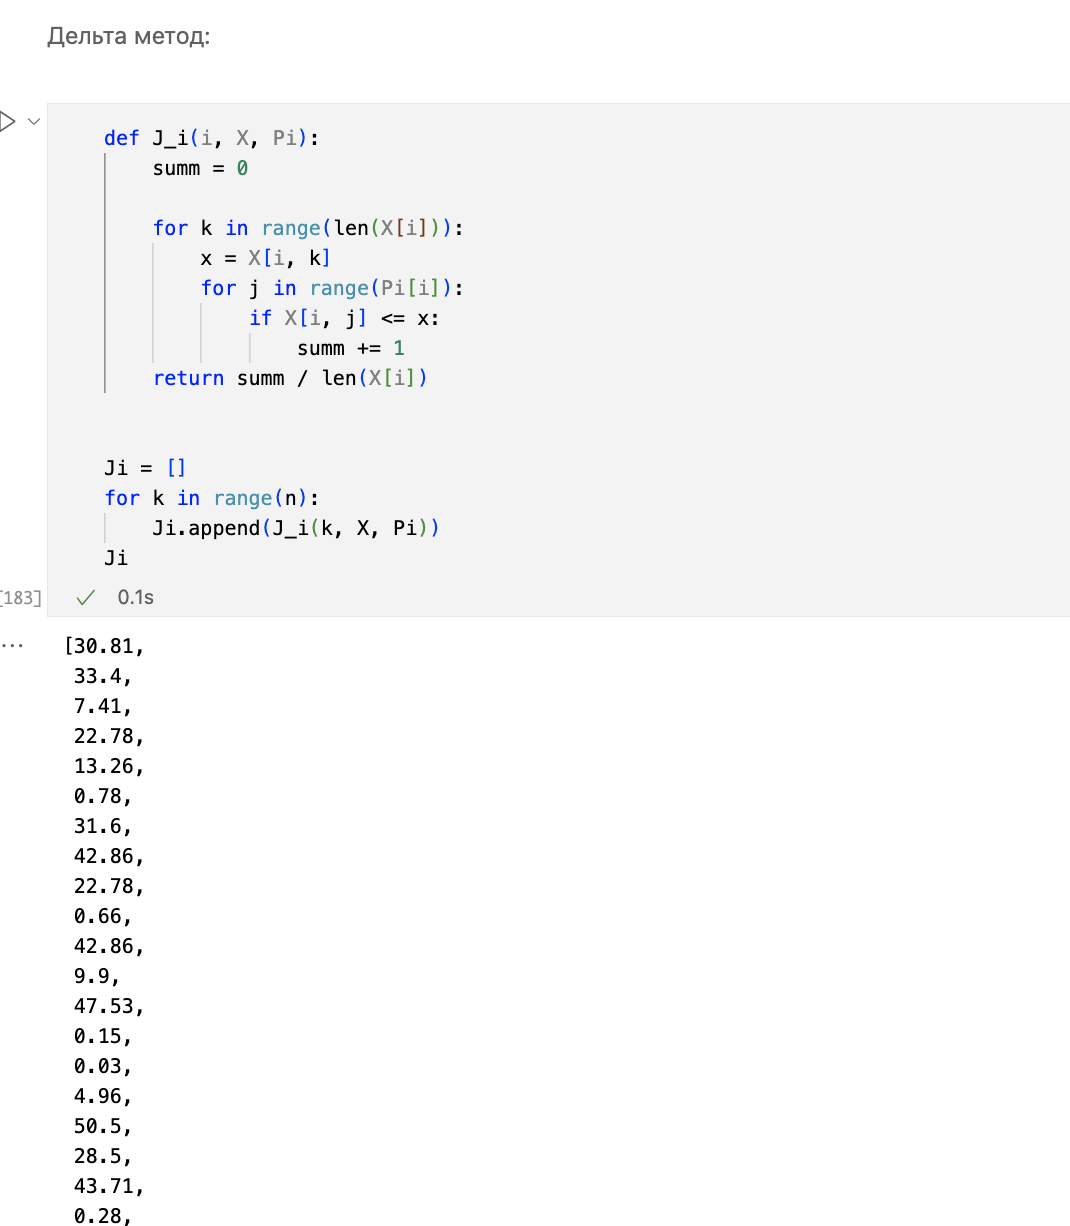
\includegraphics[width=5in]{/Users/krivonosovti/Курсач/Course_Work/Снимок экрана 2023-10-29 в 00.31.56.png}

        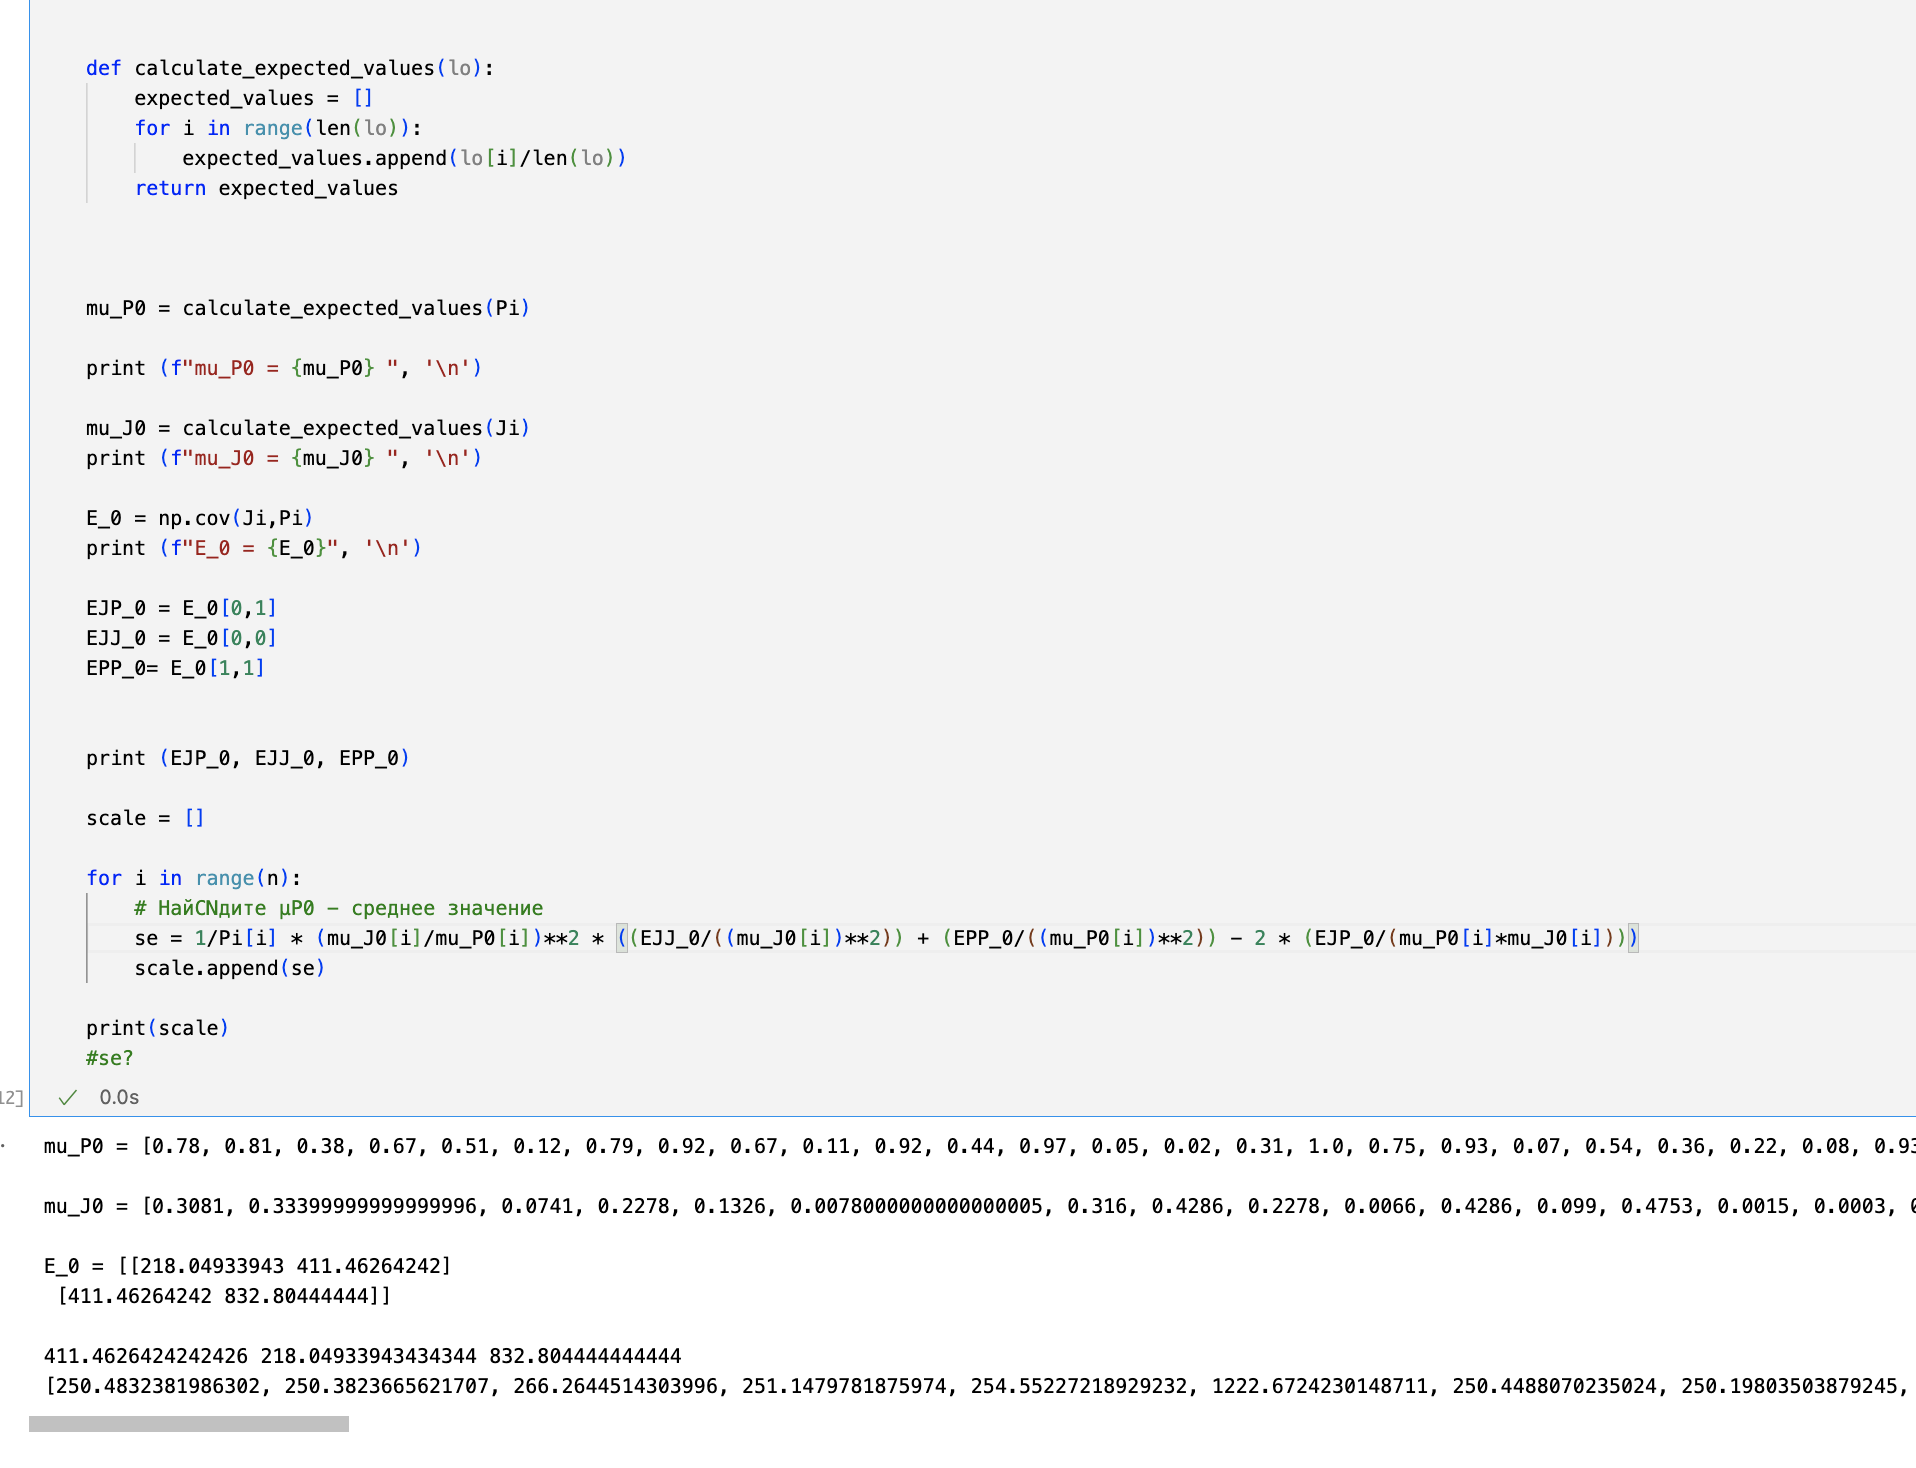
\includegraphics[width=5in]{/Users/krivonosovti/Курсач/Course_Work/Снимок экрана 2023-10-29 в 00.32.27.png}

        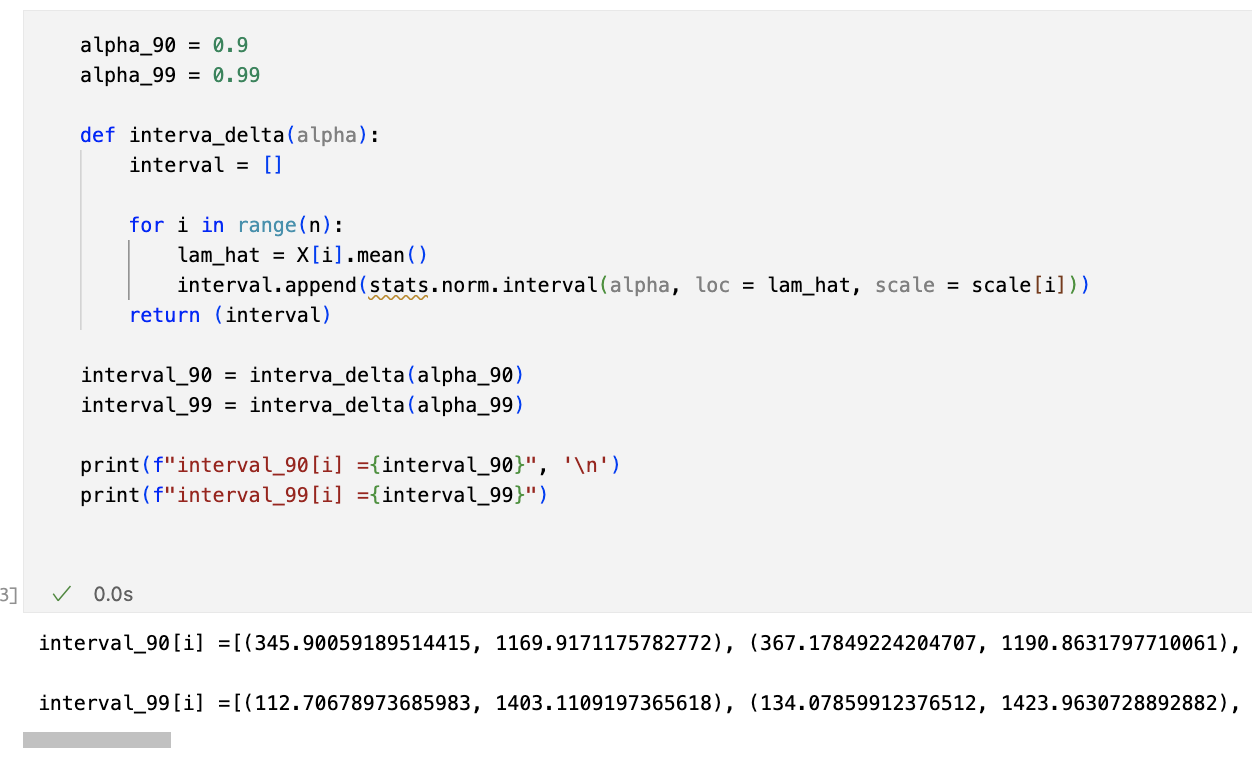
\includegraphics[width=5in]{/Users/krivonosovti/Курсач/Course_Work/Снимок экрана 2023-10-29 в 00.32.40.png}



        
        % \begin{figure}[h]
        %     \centering
        %         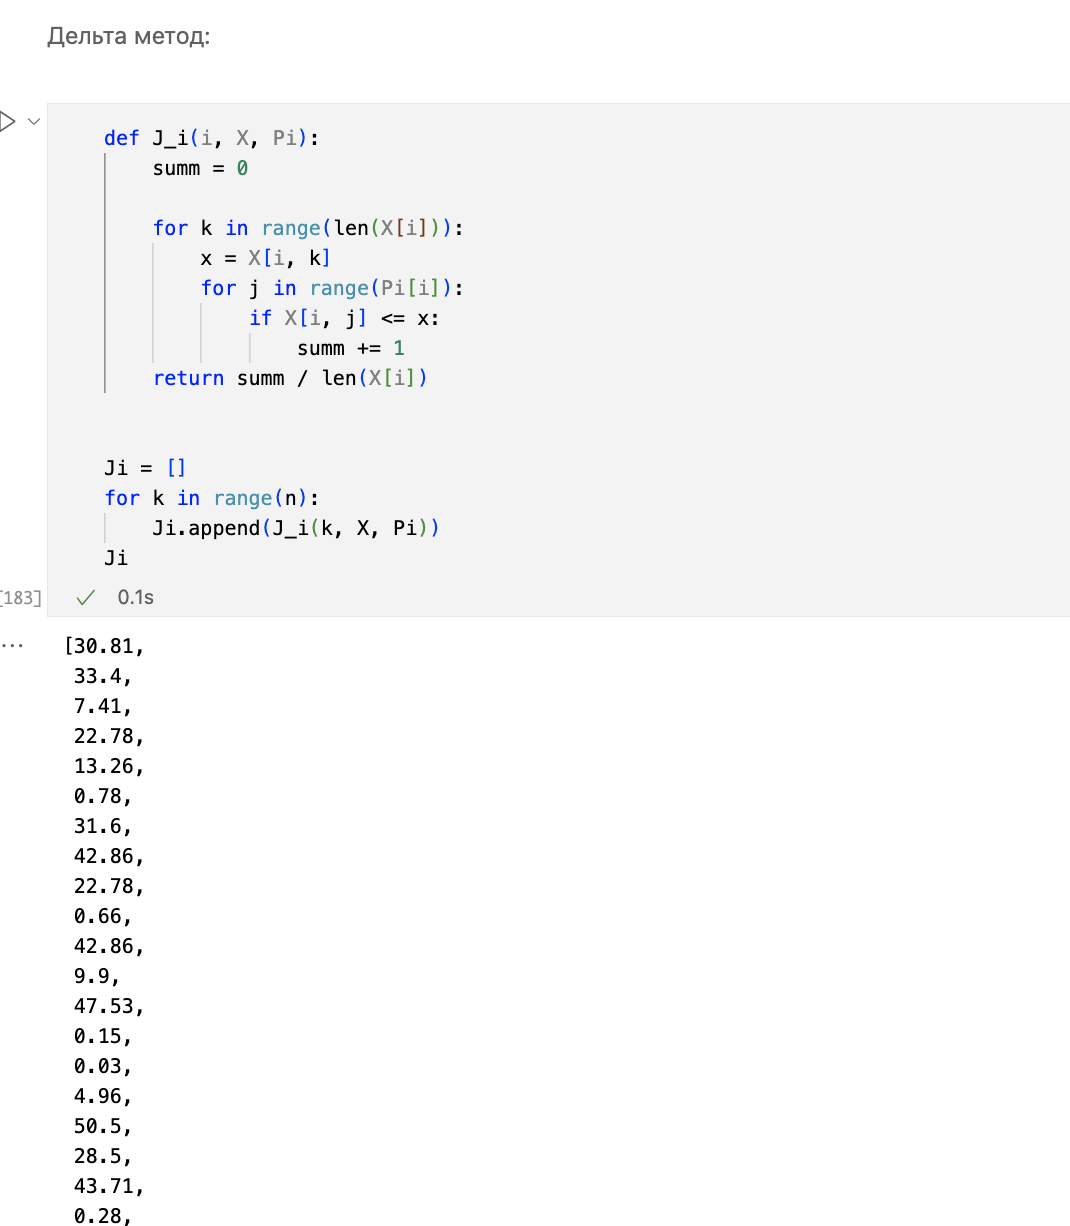
\includegraphics[width=5in]{/Users/krivonosovti/Курсач/Course_Work/Снимок экрана 2023-10-29 в 00.31.56.png}
        %         \caption{ Дельта метод. Поиск  $J_i$ }
        % \end{figure}
        % \begin{figure}[h]
        %     \centering
        %     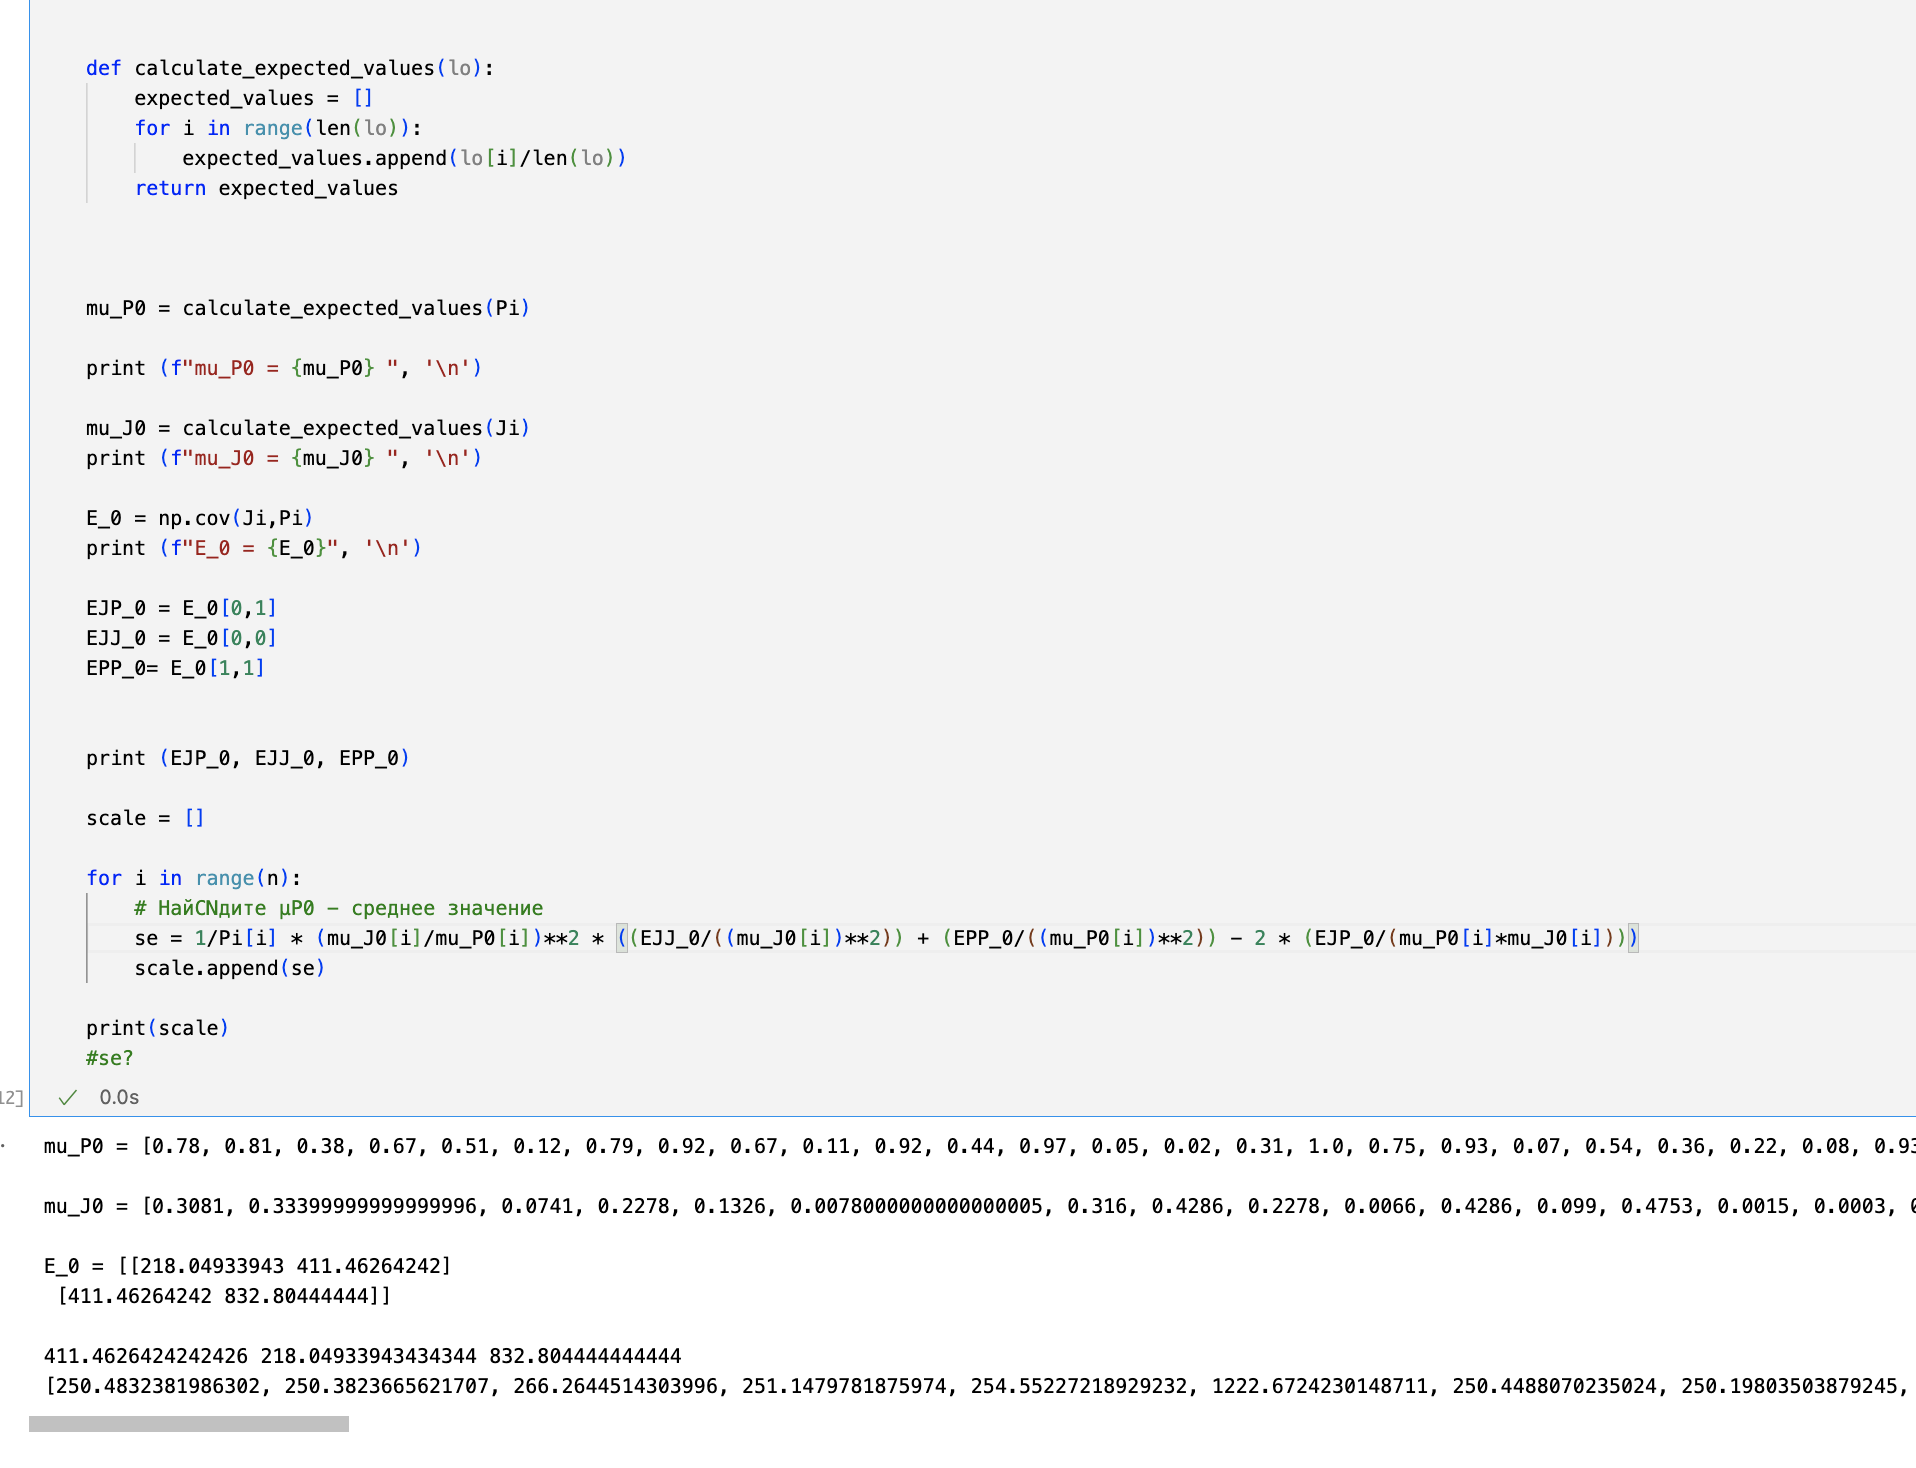
\includegraphics[width=6in]{/Users/krivonosovti/Курсач/Course_Work/Снимок экрана 2023-10-29 в 00.32.27.png}
        %     \caption{Дельта метод}
        % \end{figure}
        % \begin{figure}[h]
        %     \centering
        %         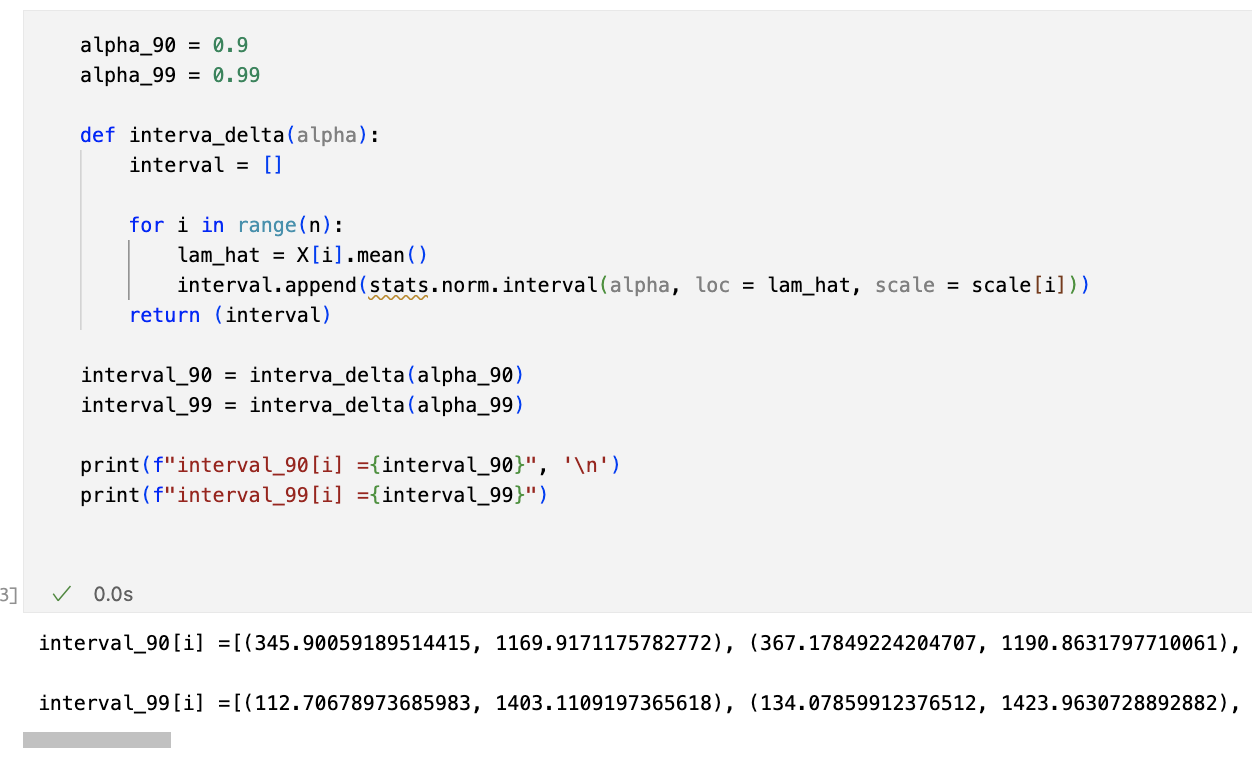
\includegraphics[width=4in]{/Users/krivonosovti/Курсач/Course_Work/Снимок экрана 2023-10-29 в 00.32.40.png}
                
        %     \caption{Резкльтат дельта метода}
        % \end{figure}



    
    \subsubsection{Подведение итогов:}

        Наивный подход, использованный для оценки доверительного интервала, показал самую слабую точность, однако при этом он остается наиболее быстрым методом. Сравнение предлагаемой методологии с использованием дельта-метода и bootstrap представлено на Рис. 7. На рисунке видно, что оценки, полученные с помощью дельта-метода и bootstrap, почти идентичны, в то время как асимптотическая оценка на Рис. 6 значительно недооценивает стандартное отклонение.

        \begin{figure}[h]
            \centering
            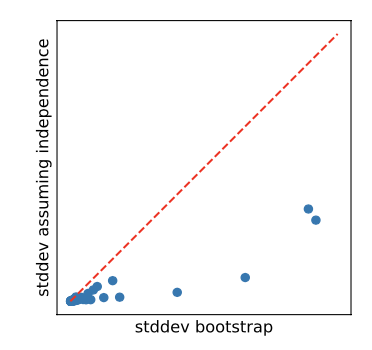
\includegraphics[width=0.5\textwidth]{/Users/krivonosovti/Курсач/Course_Work/Снимок экрана 2023-10-29 в 01.02.17.png}
            \caption{Разная оценка стандартного отклонения двух методик.  Bootstrap VS Assuming independence}
        \end{figure}
        
        \begin{figure}[h]
            \centering
            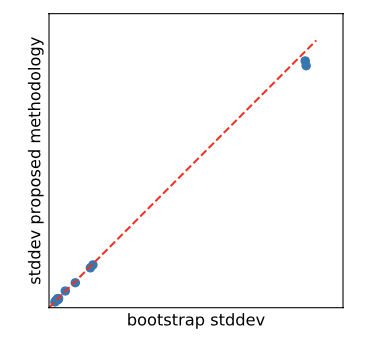
\includegraphics[width=0.5\textwidth]{/Users/krivonosovti/Курсач/Course_Work/Снимок экрана 2023-10-29 в 01.02.34.png}
            \caption{Точная оценка стандартного отклонения с предлагаемой методологией. Bootstrap VS  Proposed}
        \end{figure}


        Из полученных результатов можно сделать вывод, что дельта метод работает в 500 раз быстрее, чем бутстрэп. Однако стоит отметить, что оценка дельта метода является менее точной всего на 0.05\%. В данной задаче такая погрешность является приемлемой в пользу повышения производительности алгоритма, особенно учитывая большой объем реальных данных компаний. Необходимо отметить, что сложность алгоритма бутстрэп составляет O(nB), где B - количество повторений (приблизительно равно n). В то же время, сложность дельта метода линейна. Однако стоит заметить, что иногда сложность дельта метода может переходить в квадратичную из-за сложности вычисления градиента.

\section{Маркетинговая задача}

    \subsection{1.Основа проекта}
    Этот проект основан на данных, предоставленных на
    https://www.kaggle.com/datasets/faviovaz/marketing-ab-testing?datasetId=1660669. Это
    простая маркетинговая компания с экспериментальной и контрольной группами для A/B-
    тестирования.


    Создание A/B тестирования для dataset-а Маркетинговые компании стремятся проводить
    успешные кампании, но рынок сложен, и существует несколько вариантов, которые могут
    сработать. Поэтому обычно они проводят A/B-тестирование, которое представляет собой
    процесс случайного эксперимента, при котором две или более версии переменной (веб-
    страница, элемент страницы, баннер и т. д.) одновременно показываются разным
    сегментам людей для определения, какая версия оказывает максимальное воздействие и
    способствует достижению бизнес-метрик.
    Компании интересуются ответом на два вопроса:
    1. Сколько должно быть рекламы просмотренно человеком, чтобы с 90\% вероятностью он обратился в магазин?
    2. с 99\% вероятностью?
    С учетом второго вопроса мы обычно проводим A/B-тестирование. Большинство людей
    будут видеть рекламу (экспериментальная группа), а небольшая часть людей (контрольная
    группа) увидит общественное информирование или ничего в точно таком же размере и
    месте, где обычно размещается реклама.
    Идея этого набора данных заключается в анализе групп, определении успешности
    рекламы, оценке потенциальной прибыли от рекламы и выяснении, является ли разница
    между группами статистически значимой.

    Словарь:

    \begin{itemize}
   
        \item Index: Индекс строки
        \item user id: Идентификатор пользователя (уникальный)
        \item test group: Если "ad", то человек видел рекламу, если "psa", то он видел
        общественное информационное объявление
        \item converted: Если человек купил продукт, то значение True, иначе False
        \item total ads: Количество просмотренных рекламных объявлений человеком
        \item most ads day: День, в который человек увидел наибольшее количество рекламы
        \item most ads hour: Час дня, когда человек увидел наибольшее количество рекламы
    \end{itemize}

            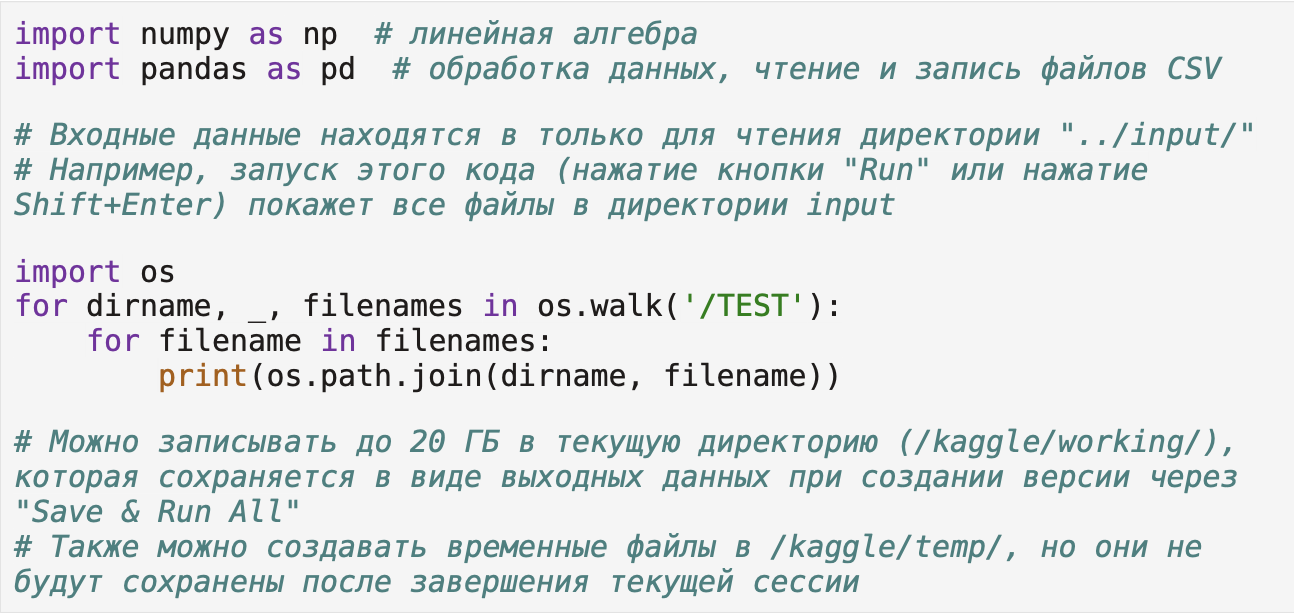
\includegraphics[width = 6in]{/Users/krivonosovti/Курсач/Course_Work/Снимок экрана 2023-10-27 в 20.47.07.png}

    \subsection{2.Подготовка данных}

    Загрузка данных


    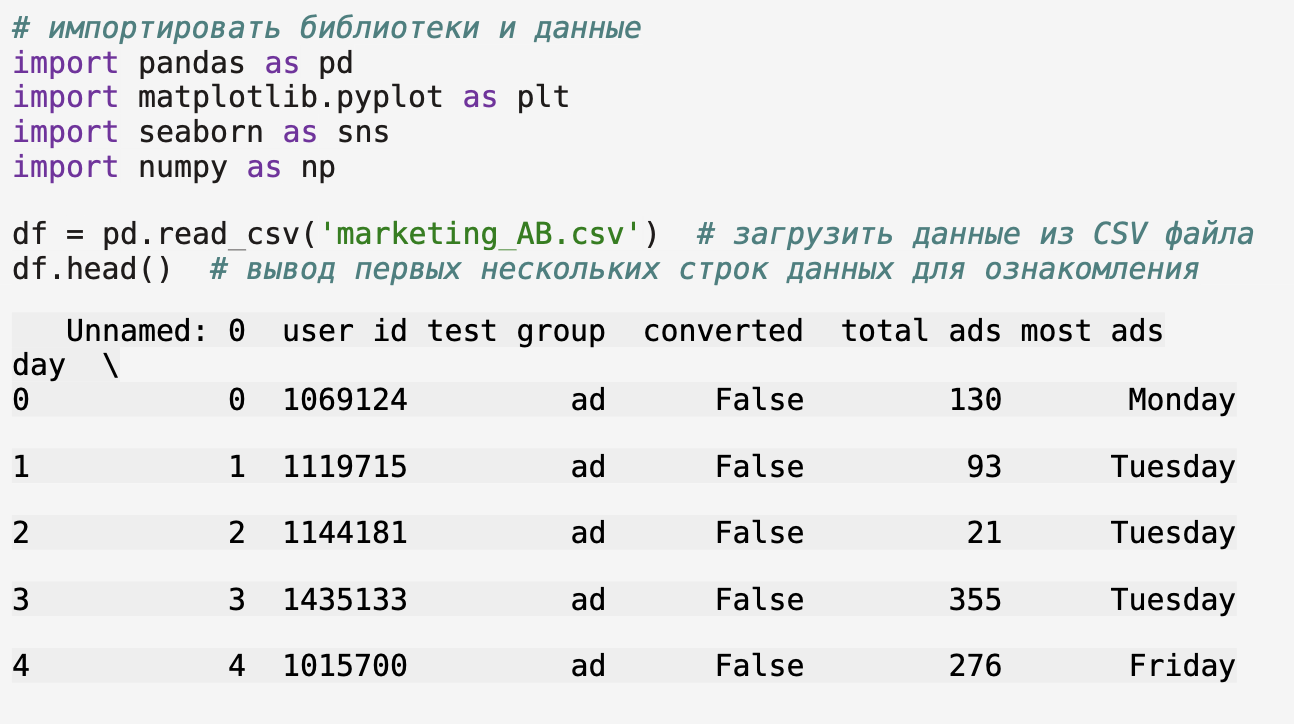
\includegraphics[width = 6in]{/Users/krivonosovti/Курсач/Course_Work/Снимок экрана 2023-10-27 в 20.47.20.png}


    После просмотра первых пяти строк таблицы данных мы обнаружили один лишний
    столбец с названием: Unnamed:0. Этот столбец нужно удалить.


    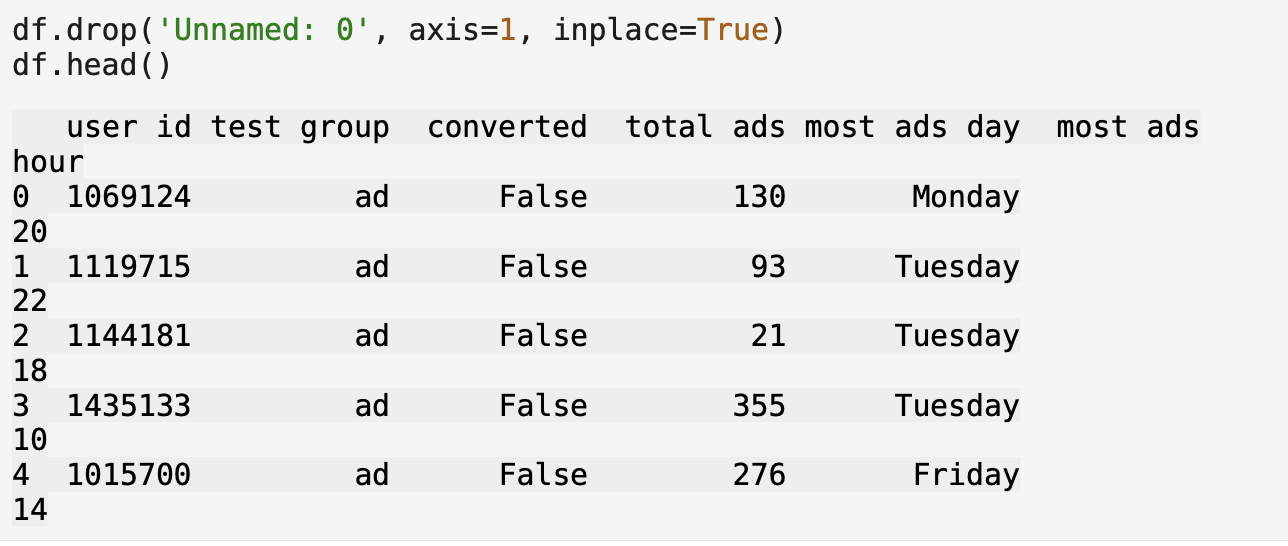
\includegraphics[width = 6in]{/Users/krivonosovti/Курсач/Course_Work/Снимок экрана 2023-10-27 в 20.47.38.png}



    После удаления столбца "Unnamed:0", текущие названия столбцов содержат пробелы между словами, 
    что может вызвать проблемы в дальнейшем. Чтобы избежать этих проблем, лучше переименовать столбец  user id в формат $user_id$.Поскольку требуется изменить большинство названий столбцов, я буду использовать 
    лямбда-функцию.


    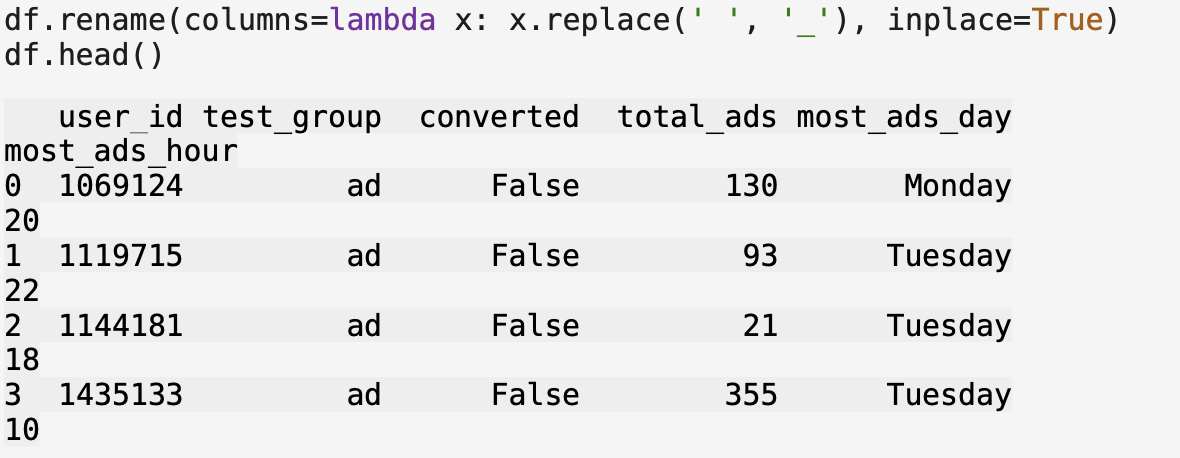
\includegraphics[width = 6in]{/Users/krivonosovti/Курсач/Course_Work/Снимок экрана 2023-10-27 в 20.47.46.png}


    Теперь датафрейм выглядит хорошо, поэтому можно проверить, есть ли пропущенные значения.


    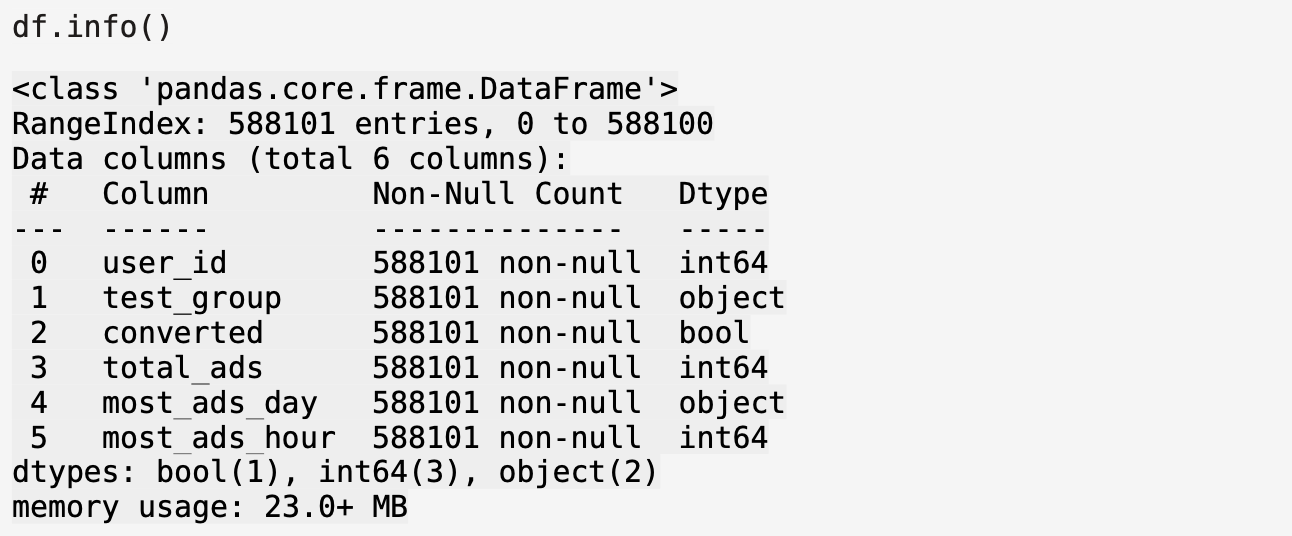
\includegraphics[width = 6in]{/Users/krivonosovti/Курсач/Course_Work/Снимок экрана 2023-10-27 в 20.47.54.png}


    К счастью, ни в одном из наших столбцов нет пропущенных значений. Вернемся к цели анализа этого 
    проекта: мы хотим узнать, значительно ли запуск рекламы улучшает конверсию. Первое, с чего следует 
    начать, это взглянуть на размер выборки экспериментальной группы (ad) и контрольной группы (psa).


    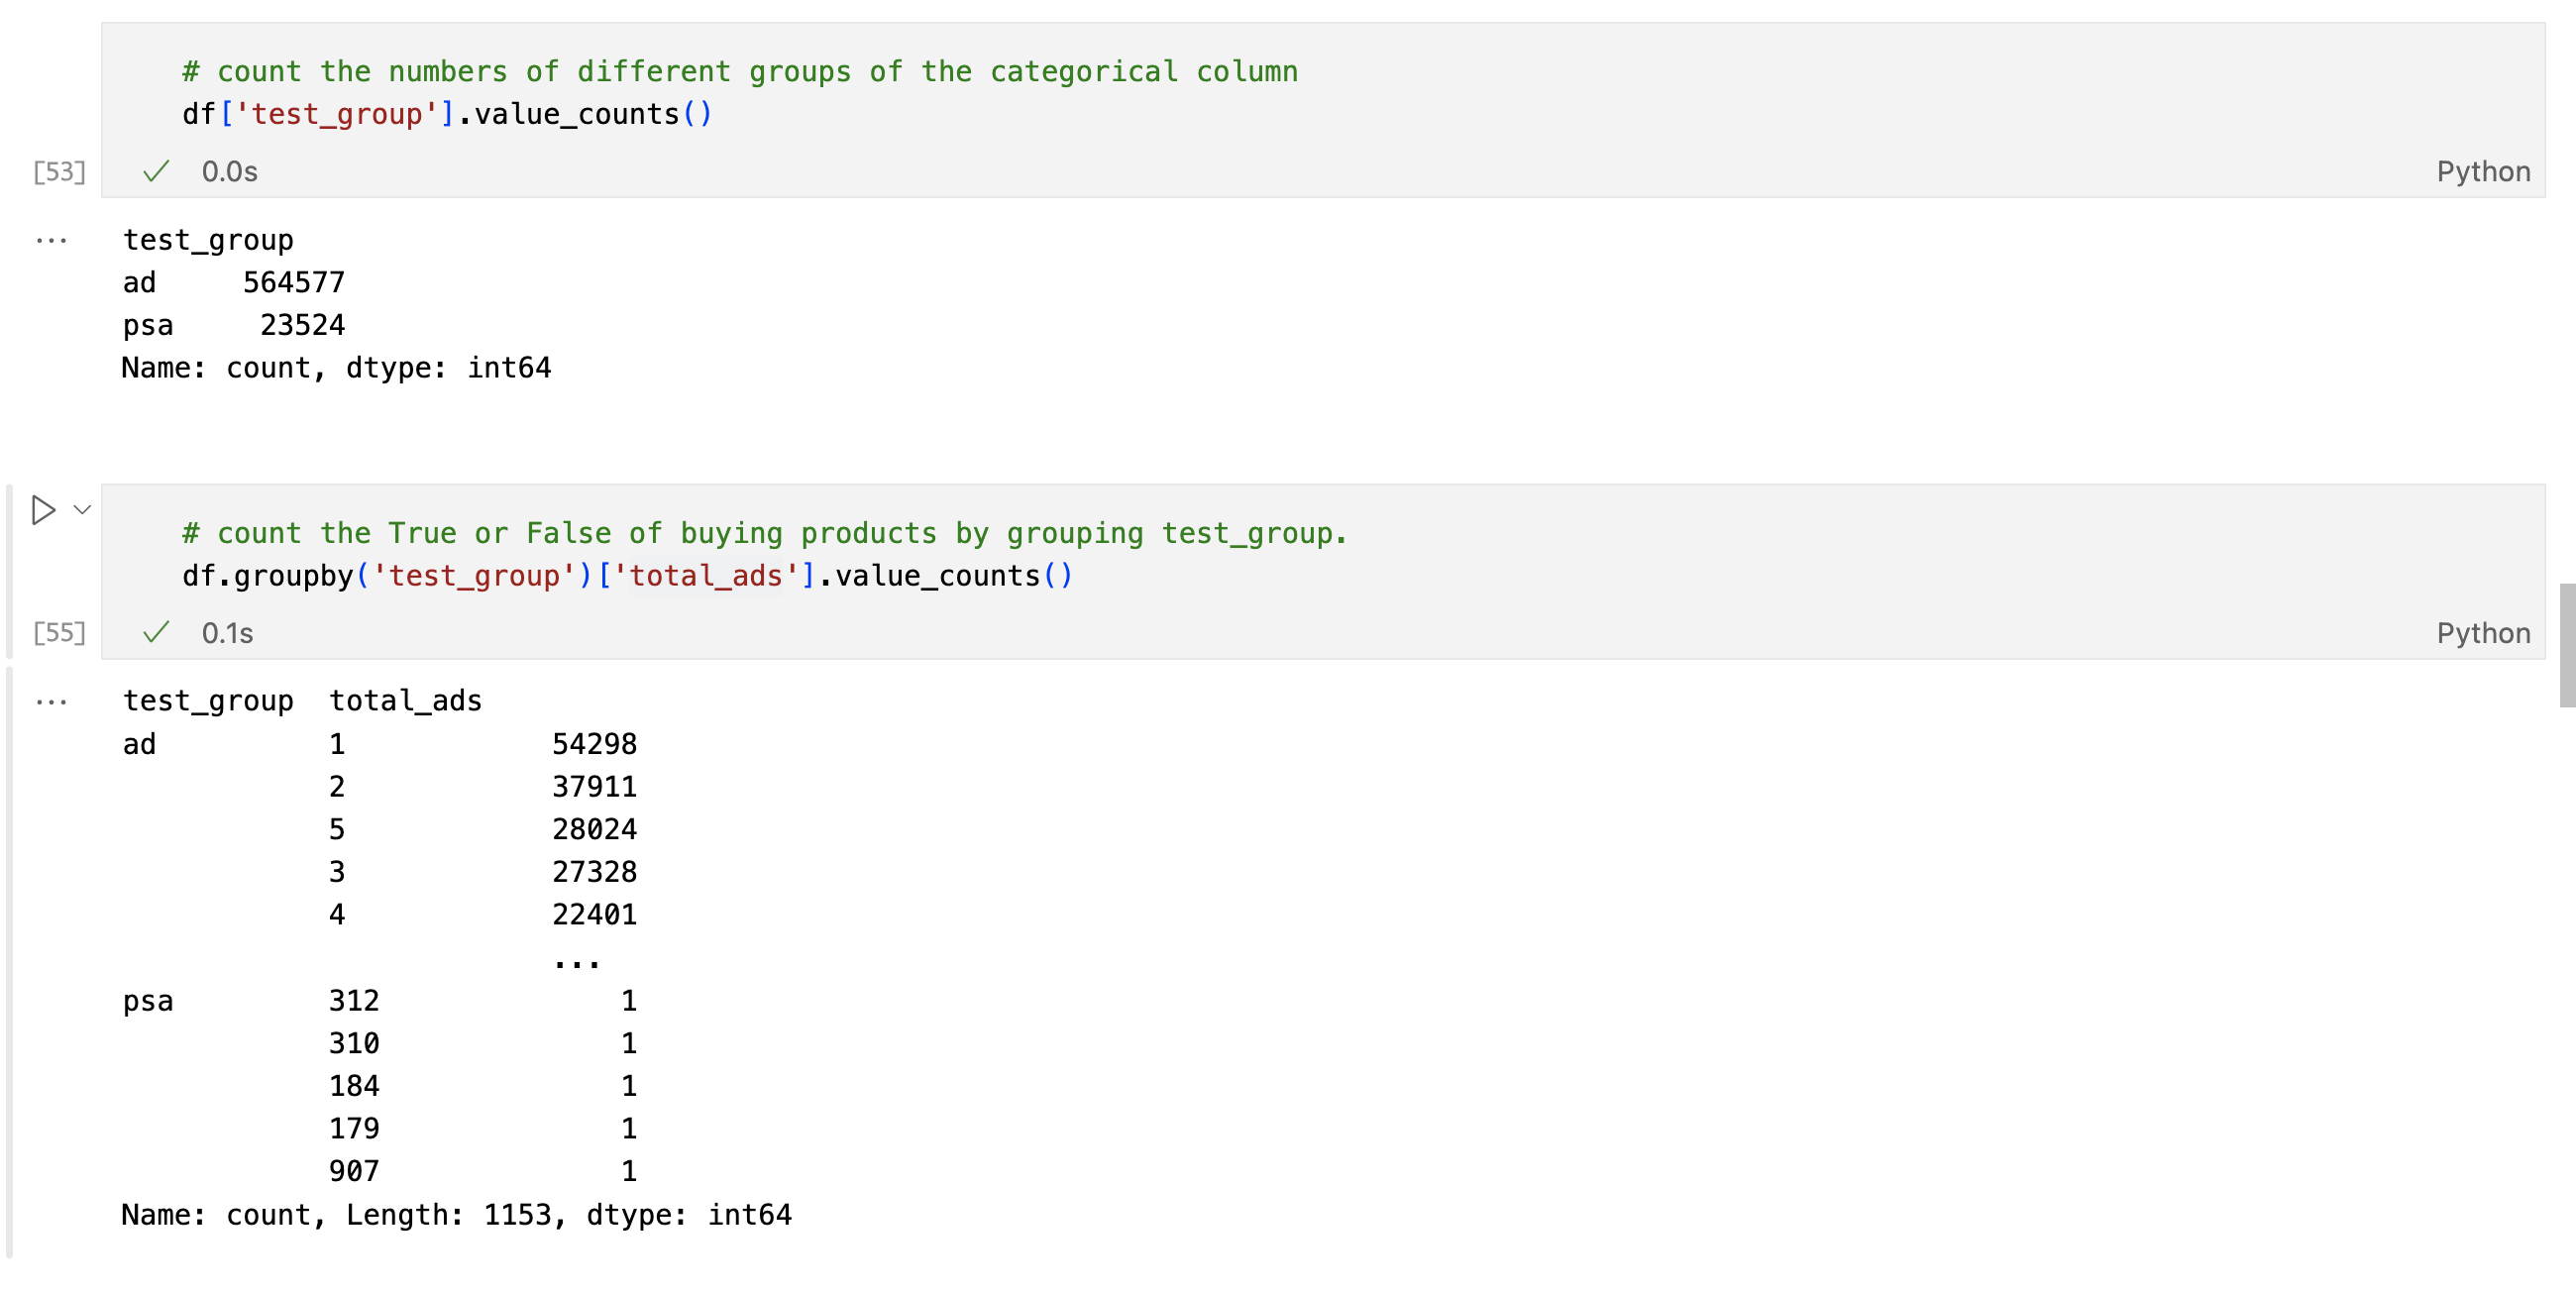
\includegraphics[width = 6in]{/Users/krivonosovti/Курсач/Course_Work/Снимок экрана 2023-10-27 в 22.23.11.png}

    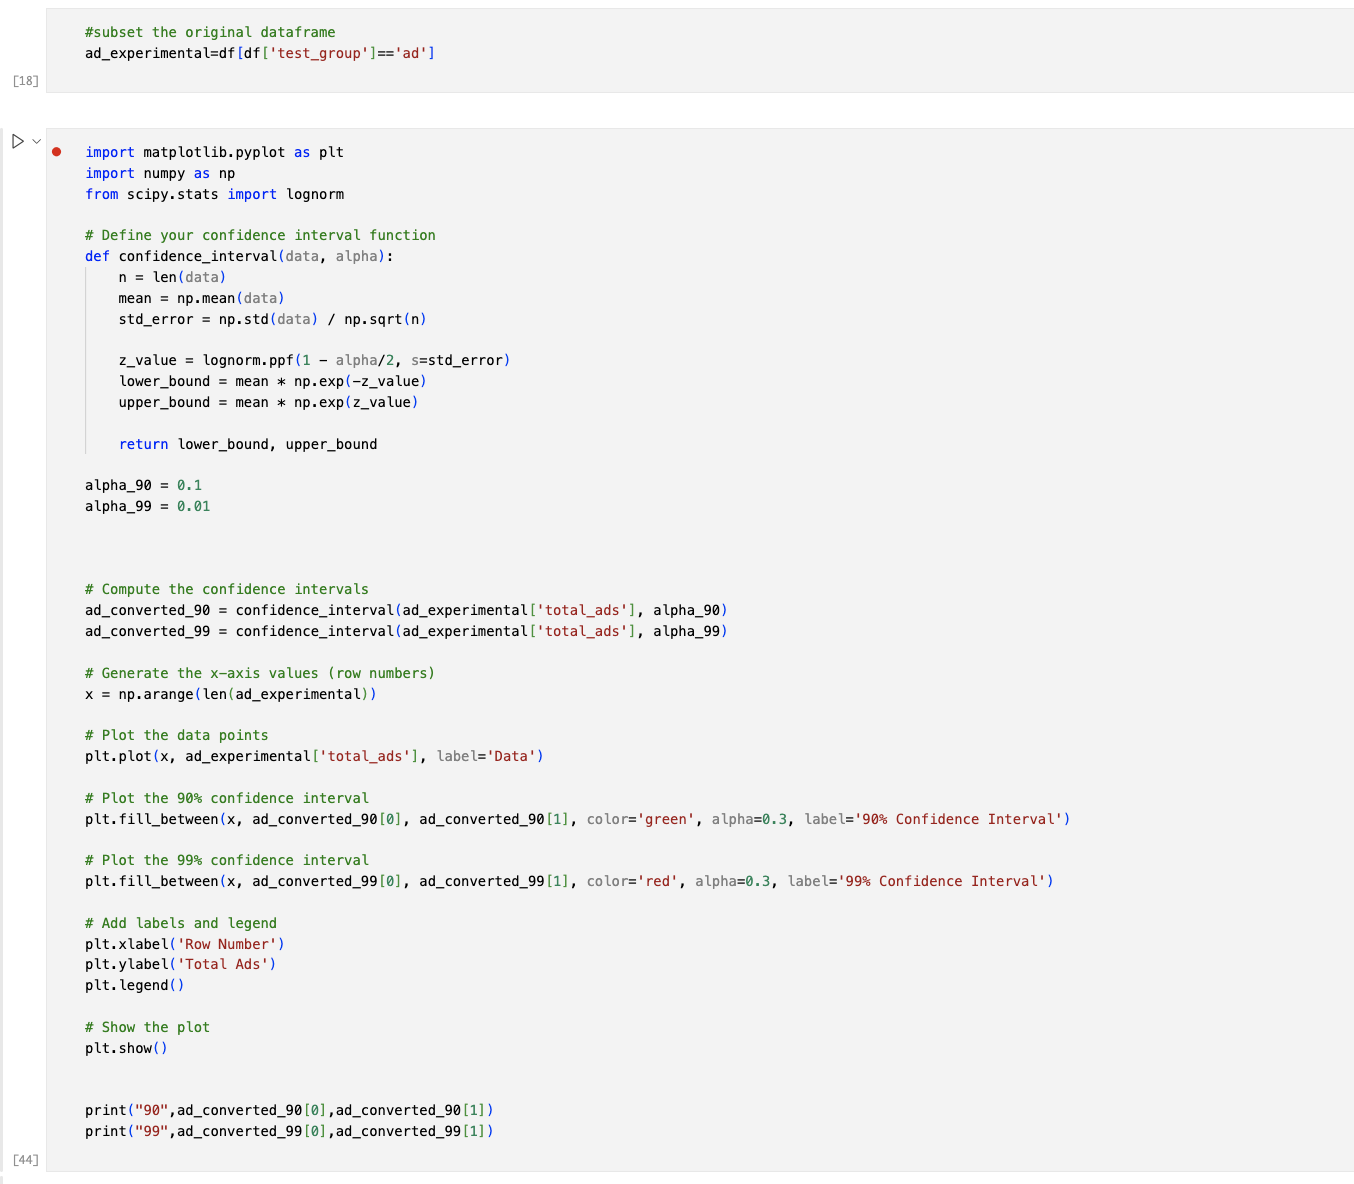
\includegraphics[width = 6in]{/Users/krivonosovti/Курсач/Course_Work/Снимок экрана 2023-10-28 в 13.59.22.png}

    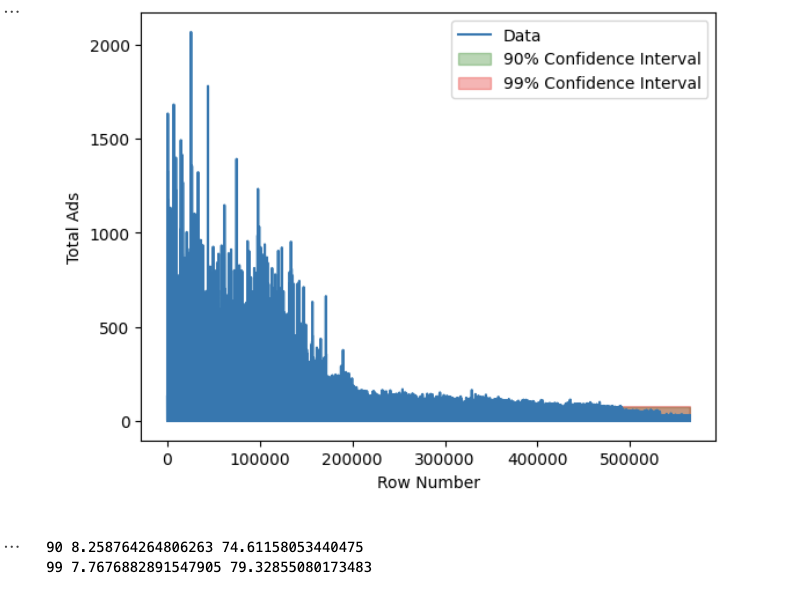
\includegraphics[width = 3in]{/Users/krivonosovti/Курсач/Course_Work/Снимок экрана 2023-10-28 в 13.59.30.png}


    Данный интервал является результатом наивного подхода. Однако, далее, при помощи метода бутстрэп, я буду стремиться улучшить его точность. 

    \subsection{Bootstrap}

    Метод bootstrap— это метод повторной выборки, используемый в статистическом анализе. По сути, он включает в себя повторную выборку наблюдений из набора данных с заменой для создания нескольких повторных выборок. Этот процесс повторной выборки позволяет оценить выборочное распределение статистики или сделать выводы о параметрах совокупности. В этом проекте я собираюсь выполнить повторную выборку исходного файла данных, чтобы создать кадры данных с повторной выборкой из 1000 выборочных средних как для экспериментальной группы, так и для контрольной группы.


    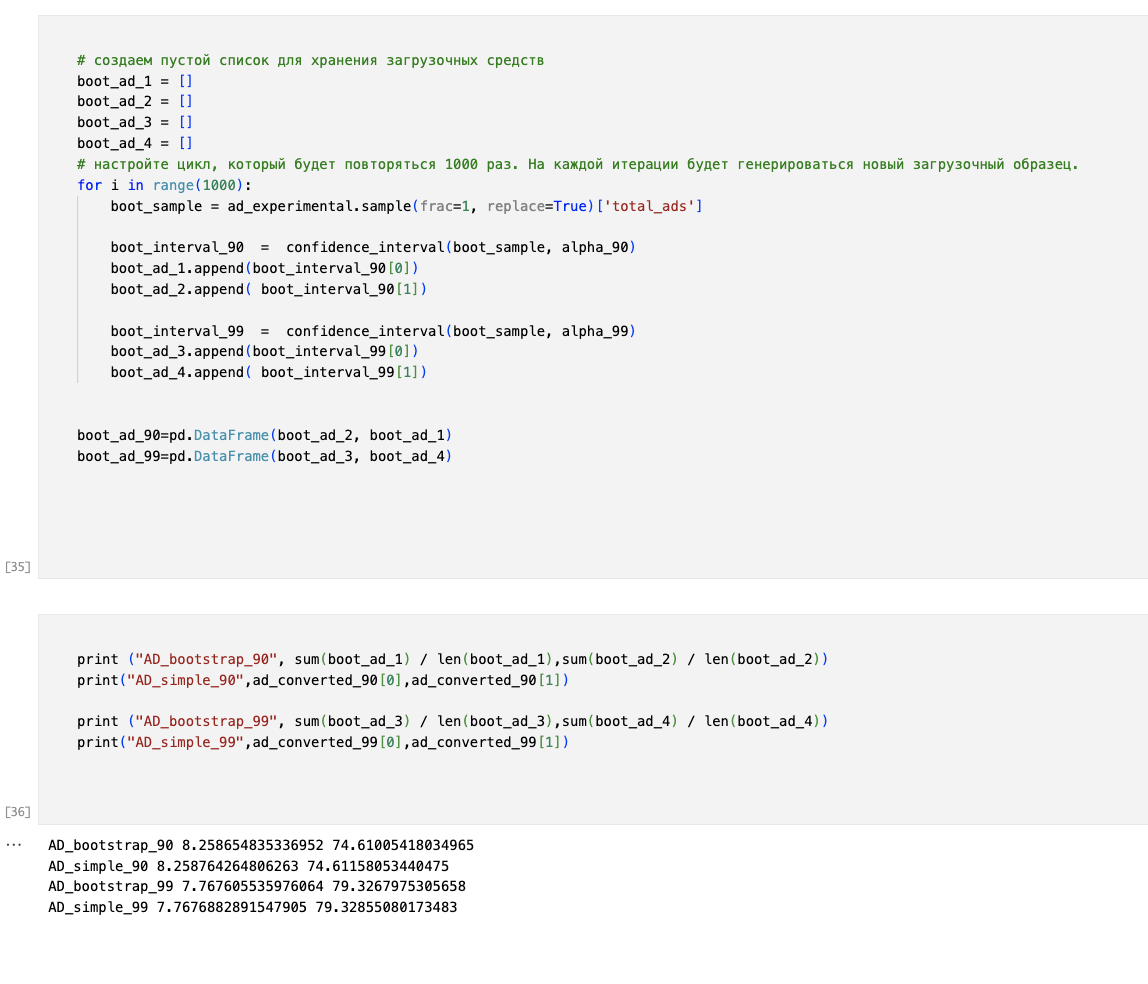
\includegraphics[width = 6in]{/Users/krivonosovti/Курсач/Course_Work/Снимок экрана 2023-10-28 в 13.59.38.png}
    

    Сравнение двух методов построения 90\% и 99\% доверительных интервалов показало, что наивный метод оказался гораздо быстрее, занимая всего 0.001 секунды, в то время как бутстрэп  для 1000 выборок занял 1 минуту и 9 секунд при использовании 500 тысяч строк данных.
    
    При анализе результатов, полученных обоими методами, наивный подход показал доверительный интервал для 90 квантиля (8.258764264806263 74.61158053440475), тогда как бутстрэп  метод выдал (8.258654835336952 74.61005418034965) для 90\% доверительного интервала. Для 99\% доверительного интервала наивный подход дал интервал (7.7676882891547905 79.32855080173483), в то время как бутстрэп  метод дал интервал (7.767713768539264 79.33688493122295).
    

   

\newpage
\section {ЗАКЛЮЧЕНИЕ}
В данной работе были представлены наиболее популярные методы, такие как bootstrap и наивный подход (все файлы курсовой можно посмотреть на \href{https://github.com/krivonosovti/QuantileCIComparison}{GitHub}). Проведено сравнение методов в задачи поиска доверительных интервалах для 90 и 99 квантилей. Также представлена статистически обоснованная и масштабируемая методология A/B-тестирования с использованием квантовых метрик (Дельта метод). Был реализован  алгоритм, основанный на этой методологии.

Подробное исследование, врешении задачи "Page loading, в также в маркетиноговой, что предложенная методология работает не менее статистически значимо, чем бутстрэп, но при этом она более чем в 500 раз быстрее, но применима не всегда.
Отвечая на главный вопрос работы о том, какой метод лучше, можно сказать, что каждый метод имеет свои преимущества в зависимости от поставленных задач. Наивный подход является быстрым, но не подходит для сложных задач. Бутстрэп, в свою очередь, не требует сложной математической базы и может быть легко адаптирован к различным задачам, однако он требует больше времени или вычислительных ресурсов. Дельта-метод наиболее применим в рассматриваемой "Page loading" задаче , но его применение усложняется требованиями к дифференцируемости вспомогательной функции и другими условиями.

Таким образом, выбор конкретного метода зависит от конкретной задачи и ее требований.

\newpage
\section {ПРИЛОЖЕНИЯ}
\begin{enumerate} 

    \item Дельта метод углубленно
        \label{sec: Приложение 1}
        Методолгия:
        Предположим, что A/B-тест задается с несколькими вариантами, где кандидаты в каждом варианте получают разный опыт. Мы заинтересованы в измерении того, как
        
        Опыт в каждом варианте влияет на q-й квантиль времени загрузки страницы. Чтобы измерить это влияние и вычислить статистическую значимость, нам нужны оценки количества выборки и стандартного отклонения квантиля выборки в каждом варианте. При увеличении одного варианта, предположим, что в этом варианте есть:
        
        Участники $i = 1,2,3,  ... , n$

        Страници просмотренные i-ым участником $j = 1, 2, 3, ... ,\textit{P}{i}$, где $\textit{P}{i}$ (i.i.d) случайные значения удовлетворяющие функции распрелеления $\mathcal{P}$.

        Загрузка j-ой страницы i-ым участником = $\textit{X}{ij}$   

        q-ый выборочный квантиль $\{\textit{X}{ij}, i = 1,2,...n; j = 1,2,3, ... ,  \textit{P}{i} \}$ обозначим как $\widehat{Q}$ 

        Дисперсия - $Var(\widehat{Q} )$; стандартное откланение $stddev(\widehat{Q})$


        
\includegraphics[width = 6in]{IMG_0086.jpg}
        \newline
        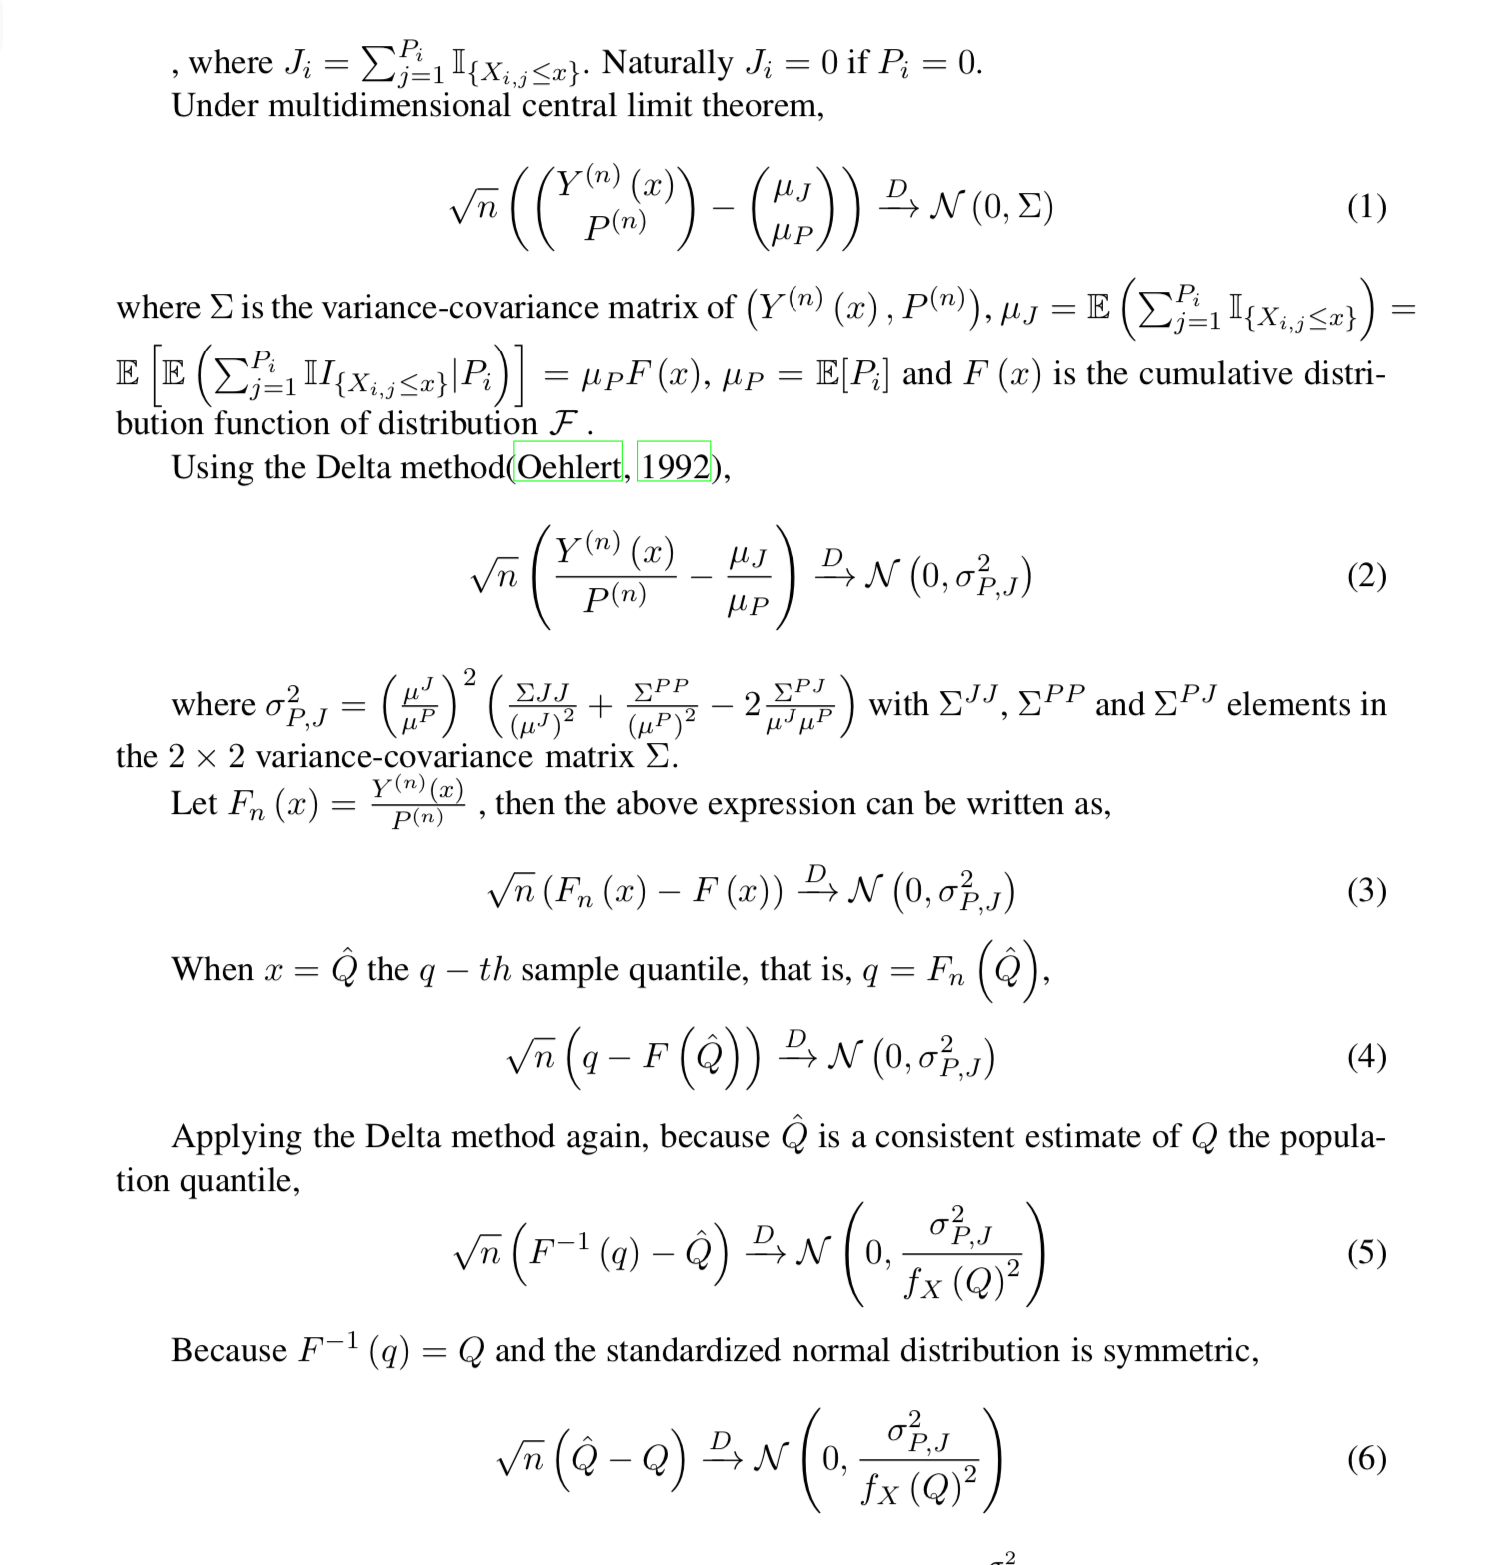
\includegraphics[width = 6in]{IMG_D1552B1059C6-1.jpeg}
        
        // тут должна быть антотация вставки 

        Таким образом асимптотическая оценка дисперисии кванитиля это $\frac{\sigma ^ 2_{P,J}}{nf_{X}(Q)^2}$,  где Q можно оценить со средней плотностью в небольшом доверительном интевале $\widehat{Q}$.

        Предположим, что из n участников только  $i = 1, 2,...,n_0$  имет ненулевые просмотры на интересующей странице.
        
        Определим: 
        
        $\mu_0^J = E(J_i|i =1,2, ... , n_0)$; $\mu_0^P = E(P_i|i =1,2, ... , n_0)$; $\Sigma_0 = Cov(J_i,P_i|i = 1,2,...,n_0)$
        Тогда:

        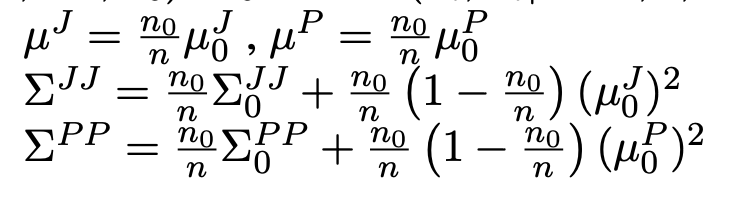
\includegraphics[width = 3in]{Снимок экрана 2023-10-16 в 22.09.59.png}

        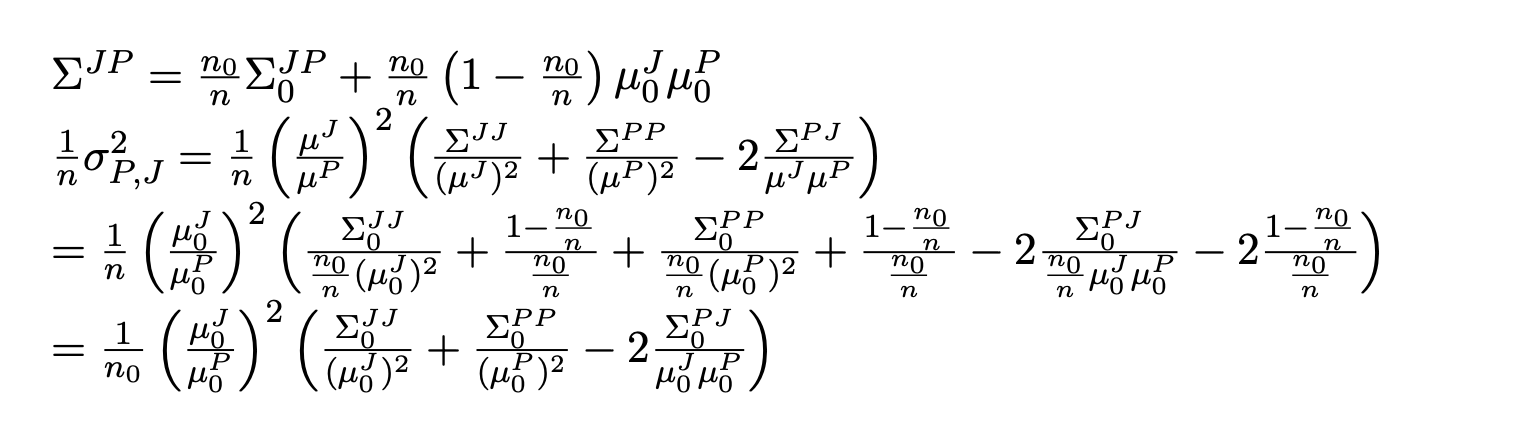
\includegraphics[width = 6in]{Снимок экрана 2023-10-16 в 22.10.53.png}

        Источник \textit{"Large-Scale Online Experimentation with Quantile Metric"} Min Liu, Xiaohui Sun, Maneesh Varshney, Ya Xu. [Online]. Available: \url{https://arxiv.org/abs/1903.08762v1}.
\end{enumerate}
\newpage
\section{ИСТОЧНИКИ}
\begin{itemize}
        \item \textit{"Large-Scale Online Experimentation with Quantile Metric"} Min Liu, Xiaohui Sun, Maneesh Varshney, Ya Xu. [Online]. Available: \url{https://arxiv.org/abs/1903.08762v1}
    
        \item \textit{"Applying the Delta method in metric analytics: A practical guide with novel ideas"} Alex Deng, Ulf Knoblich, Jiannan Lu. [Online]. Available: \url{https://arxiv.org/abs/1803.06336v4}
    
        \item Лекции Computer Science Center
    
        \item Wikipedia. [Online]. Available: \url{https://en.wikipedia.org/wiki/Main_Page}
    
        \item OpenAI. [Online]. Available: \url{https://openai.com}
    
        \item Книга \textit{"Trustworthy Online Controlled Experiments: A Practical Guide to A/B Testing"} Ron Kohavi, Diane Tang, Ya Xu.
\end{itemize}
        
\end{document}